\documentclass{cmc}
\usepackage{subcaption}
\usepackage{mathtools}

\begin{document}

\pagestyle{fancy}
\lhead{\textit{\textbf{Computational Motor Control, Spring 2018} \\
    Python exercise, Lab 5, GRADED}} \rhead{Freundler, Freundler, Wang}

\section*{Student names: Frederic Freundler, Ndicolas Freundler, Ruijia Wang}

\textit{Instructions: Update this file (or recreate a similar one,
  e.g.\ in Word) to prepare your answers to the questions. Feel free
  to add text, equations and figures as needed. Hand-written notes,
  e.g.\ for the development of equations, can also be included e.g.\
  as pictures (from your cell phone or from a scanner).
  \textbf{\corr{This lab is graded.}} and need to be submitted before
  the \textbf{\corr{Deadline : 23-04-2018 Midnight}}.  \\ Please
  submit both the source file (*.doc/*.tex) and a pdf of your
  document, as well as all the used and updated Python functions in a
  single zipped file called \corr{lab5\_name1\_name2\_name3.zip} where
  name\# are the team member’s last names.  \corr{Please submit only
    one report per team!}}
\\

In the previous week you explored the behavior of a simple pendulum
model with passive elements such as springs and dampers and then
explored the properties of a single but more realstic muscle model
with both active and passive components.

The main goal of this exercise is to explore the behavior of the
pendulum model attached with two antagonist Hill-type muscles and then
connect a half-center neural network model to drive the muscles in the
pendulum. The system is as shown in figure \ref{fig:p_muscles}.

\subsection*{Files to complete the exercises}
\label{sec:intro}

\begin{itemize}
\item \fileref{lab5.py} : Main file
\item \fileref{exercise3.py} : Main file to complete exercise 3
\item \fileref{exercise4.py} : Main file to complete exercise 4
\item \fileref{SystemParameters.py} : Parameter class for Pendulum,
  Muscles and Neural Network (Create an instance and change properties
  using the instance. You do not have to modify the file)
\item \fileref{Muscle.py} : Muscle class (You do not have to modify
  the file)
\item \fileref{System.py} : System class to combine different models
  like Pendulum, Muscles, Neural Network (You do not have to modify
  the file)
\item \fileref{PendulumSystem.py} : Contains the description of
  pendulum equation and Pendulum class. You can use the file to define
  perturbations in the pendulum.
\item \fileref{MuscleSystem.py} : Class to combine two muscles (You do
  not have to modify the file)
\item \fileref{NeuralSystem.py} : Class to describe the neural network
  (You do not have to modify the file)
\item \fileref{SystemSimulation.py} : Class to initialize all the
  systems, validate and to perform integration (You do not have to
  modify the file)
\item \fileref{SystemAnimation.py} : Class to produce animation of the
  systems after integration (You do not have to modify the file)
\end{itemize}

\textbf{NOTE : } '\textit{You do not have to modify}' does not mean
you should not, it means it is not necessary to complete the
exercises. But, \corr{you are expected to look into each of these
  files and understand how everything works}. You are free to explore
and change any file if you feel so.

\section*{Exercise 3 : Pendulum model with Muscles}
\label{sec:question-1}

\begin{figure}[H]
  \centering \includegraphics[scale=1.0]{figures/pendulum_muscles.pdf}
  \caption{Pendulum with Antagonist Hill Muscles}
  \label{fig:p_muscles}
\end{figure}

The system is comprised of a physical pendulum described by equation \ref{eq:pendulum} and a pair of antagonist muscles \textbf{M1} and \textbf{M2}. Muscle \textbf{M1} extends the pendulum ($\theta$ decreases) and Muscle \textbf{M2} flexes the muscle ($\theta$ increases).

Consider the system only for the pendulum range $\theta$ =
$[-\pi/2, \pi/2]$

\begin{equation}
  \label{eq:pendulum}
  I\ddot{\theta} = - m \cdot g \cdot L \cdot sin(\theta)
\end{equation}

Where,

\begin{itemize}
\item $I$ - Pendulum inertia about the pendulum pivot joint
  [$kg \cdot m^2$]
\item $\theta$ - Pendulum angular position with the vertical [$rad$]
\item $\ddot{\theta}$ - Pendulum angular acceleration
  [$rad \cdot s^{-2}$]
\item $m$ - Pendulum mass [$kg$]
\item $g$ - System gravity [$m \cdot s^{-2}$]
\item $L$ - Length of the pendulum [$m$]
\end{itemize}

Each muscle is modelled using the Hill-type equations that you are now
familiar with.  Muscles have two attachment points, one at the origin
and the other at the insertion point.  The origin points are denoted
by $O_{1,2}$ and the insertion points by $I_{1,2}$. The two points of
attachment dictate how the length of the muscle changes with respect
to the change in position of the pendulum.

The active and passive forces produced by the muscle are transmitted
to the pendulum via the tendons. In order to apply this force on to
the pendulum, we need to compute the moment based on the attachments
of the muscle.

Using the laws of sines and cosines, we can derive the length of
muscle and moment arm as below. The reference to the paper can be found here
\href{https://www.ncbi.nlm.nih.gov/pmc/articles/PMC5323435}{\corr{Reference}},

\begin{eqnarray}
  \label{eq:2}
  L_1 = \sqrt[2]{a_{1}^2 + a_{2}^2 + 2 \cdot a_1 \cdot a_2 \cdot \sin(\theta)} \\
  h_1 = \frac{a_1 \cdot a_2 \cdot \cos(\theta)}{L_1}
\end{eqnarray}

Where,

\begin{itemize}
\item $L_1$ : Length of muscle 1
\item $a_1$ : Distance between muscle 1 origin and pendulum origin
  ($|O_1C|$)
\item $a_2$ : Distance between muscle 1 insertion and pendulum origin
  ($|I_1C|$)
\item $h_1$ : Moment arm of the muscle
\end{itemize}

\begin{figure}[H]
  \centering
  \includegraphics[scale=1]{figures/pendulum_muscles_force_length.pdf}
  \caption[force_length]{Computation of muscle length and moment arm}
  \label{fig:pendulum_muscles_force_length}
\end{figure}

Equation \ref{eq:2} can be extended to the Muscle 2 in similar
way. Thus, the final torque applied by the muscle on to the pendulum
is given by,

\begin{equation}
  \label{eq:3}
  \tau = F \cdot h
\end{equation}

Where,

\begin{itemize}
\item $\tau$ : Torque [$N \cdot m$]
\item $F$ : Muscle Tendon Force [$N$]
\item $h$ : Muscle Moment Arm [$m$]

\end{itemize}

In this exercise, the following states of the system are integrated
over time,

\begin{equation}
  \label{eq:0}
  X = \begin{bmatrix}
    \theta & \dot{\theta} & A_1 & l_{CE1} & A_2 & l_{CE2}
  \end{bmatrix}
\end{equation}

Where,

\begin{itemize}
\item $\theta$ : Angular position of the pendulum [rad]
\item $\dot{\theta}$ : Angular velocity of the pendulum [rad/s]
\item $A_1$ : Activation of muscle 1 with a range between [0, 1].  0
  corresponds to no stimulation and 1 corresponds to maximal
  stimulation.
\item $l_{CE1}$ : Length of contracticle element of muscle 1
\item $A_2$ : Activation of muscle 2 with a range between [0, 1].  0
  corresponds to no stimulation and 1 corresponds to maximal
  stimulation.
\item $l_{CE2}$ : Length of contracticle element of muscle 2
\end{itemize}

To complete this exercise you will make use of the following files,
\fileref{exercise3.py}, \fileref{SystemParameters.py},
\fileref{Muscle.py}, \fileref{System.py}, \fileref{PendulumSystem.py},
\fileref{MuscleSystem.py}, \fileref{SystemSimulation.py}

\label{sec:questions}

\subsection*{3a. For a given set of attachment points, compute and
  plot the muscle length and moment arm as a function of $\theta$
  between $[-\pi/2, \pi/2]$ using equations in \corr{eqn:\ref{eq:2}}
  and discuss how it influences the pendulum resting position and the
  torques muscles can apply at different joint angles.}
\label{sec:3a}

For this first exploration of the model, we decided to compute, for each of five origin points of the two muscles and four insertion positions. Origin points are placed from 0.01 to 0.2 m apart from the pendulum's pivot which is also the origin of the system, so that the insertion for the left muscle (i.e. $M1$) are in the negative direction. The insertion positions are placed from 0.15 to 0.3 m from the pendulum's pivot, also in the negative direction.

For each simulation, we used a heavy weighted pendulum and started it at a position of $\pi/2 - \epsilon$ to make sure that its trajectory would cover the interval [$-\pi/2, \pi/2$]. Since the exact $-\pi/2$ and $\pi/2$ values are not defined in the model, we approach them by $\epsilon$ (a small value) and never properly reach them. We plotted left muscle's ($M1$) length and moment arm in Figures \ref{figure:3_1a}, \ref{figure:3a_1_follow} and \ref{figure:3a_1_end}, but the results would be the same for the right muscle ($M2$), since both muscles share the same characteristics, and are set with an activity of 0.05 throughout the entire simulation.

For origins at -0.01 and 0.01 m, which are very close to the pendulum's pivot point, we observe that over the whole range ([$-\pi/2, \pi/2$]), the muscle length won't deviate much from the value corresponding to the insertion distances, which seems logical: the closer the muscle's origin point is to the pivot, the more it resembles the pendulum itself, with a length corresponding to the insertion distance. Concerning the length, another observation, valid for every value of muscle origin, is that when the pendulum is at position $\sim\pi/2$, the muscle length for $M1$ is equal to the sum of the absolute value of origin and the absolute insertion value $\vert O_1\vert + \vert I_1\vert$. Conversely, when the pendulum is at position $\sim-\pi/2$, $M1$'s length is equal to $\bigr\rvert\vert I_1\vert - \vert O_1\vert\bigr\rvert$. These identities work the other way around for $M2$. Note that when the origin is set at $O_1 = -0.15$ m and the insertion at the same value (see Figure \ref{figure:3a_1_follow} bottom, blue), we reach a muscle length of 0.0, consistently with our understanding of the model. Interestingly, even for a heavy pendulum weight as is the case here, when we go above a certain set of origin points, the pendulum doesn't cover the whole angular range for each and every insertion point (see Figures \ref{figure:3a_1_follow} bottom and \ref{figure:3a_1_end}). This is due to the increased moment arm of both muscles, meaning that the opposite muscle $M2$ has a greater ability to retain the pendulum from going all the way towards the opposite direction.

Concerning these moment arms, displayed on the right side of each sub-figure, the first thing to notice is their bell shaped dynamics, and the fact that the maximal value they display is equal to the absolute distance of origin of the muscle $\vert O_1\vert$. This is consistent with the model's design: the moment arms correspond to the orthogonal projection on the muscle, passing through the pivot point, and can never be greater than the $\vert O_1\vert$ origin distance. It is thus equal to $\vert O_1\vert$ -- and maximal -- when the muscle is vertical. For every case where $\vert O_1\vert\neq\vert I_1\vert$, $-\pi/2$ and $\pi/2$ correspond to a null moment arm, because the moment arm is along the pendulum itself, so it can't have any physical action on it. In the case where $\vert O_1\vert$ = $\vert I_1\vert$, as in Figure \ref{figure:3a_1_follow} bottom, blue or Figure \ref{figure:3a_1_end}, orange, the muscle would be vertical and the moment arm maximal at $\sim-\pi/2$, but would automatically drop to 0.0 at the exact value, should it be defined in the computation, which is not the case here.

\newpage
About the maximal values of the moment arms, one can see that the closest from the pivot point the origin is set, the more the muscle is quasi-vertical near 0.0 radians, as in Figure \ref{figure:3_1a} top, and the maximum arm value will then be around that position too. When we move the $O_1$ point farther from the pivot point, we stretch the maximum moment arm to the right -- or to the left if we consider the $M2$ muscle. Also noticeable is the fact that when $\vert O_1\vert > \vert I_1\vert$, as in Figure \ref{figure:3a_1_end}, blue, the muscle can never be vertical within the [$-\pi/2, \pi/2$] interval, such that the maximum moment arm will never be equal to $\vert O_1\vert$.

Finally, the bell shape of the dynamics, especially its steepening slope when going towards the range boundaries $-\pi/2$ and $\pi/2$, is responsible for the fact that the rate of length/position is lower towards these values, as testifies the sigmoid dynamics of the muscle length. It means that the length changing rate diminishes as does the moment arms.

\begin{figure} [H]
\centering
{%
  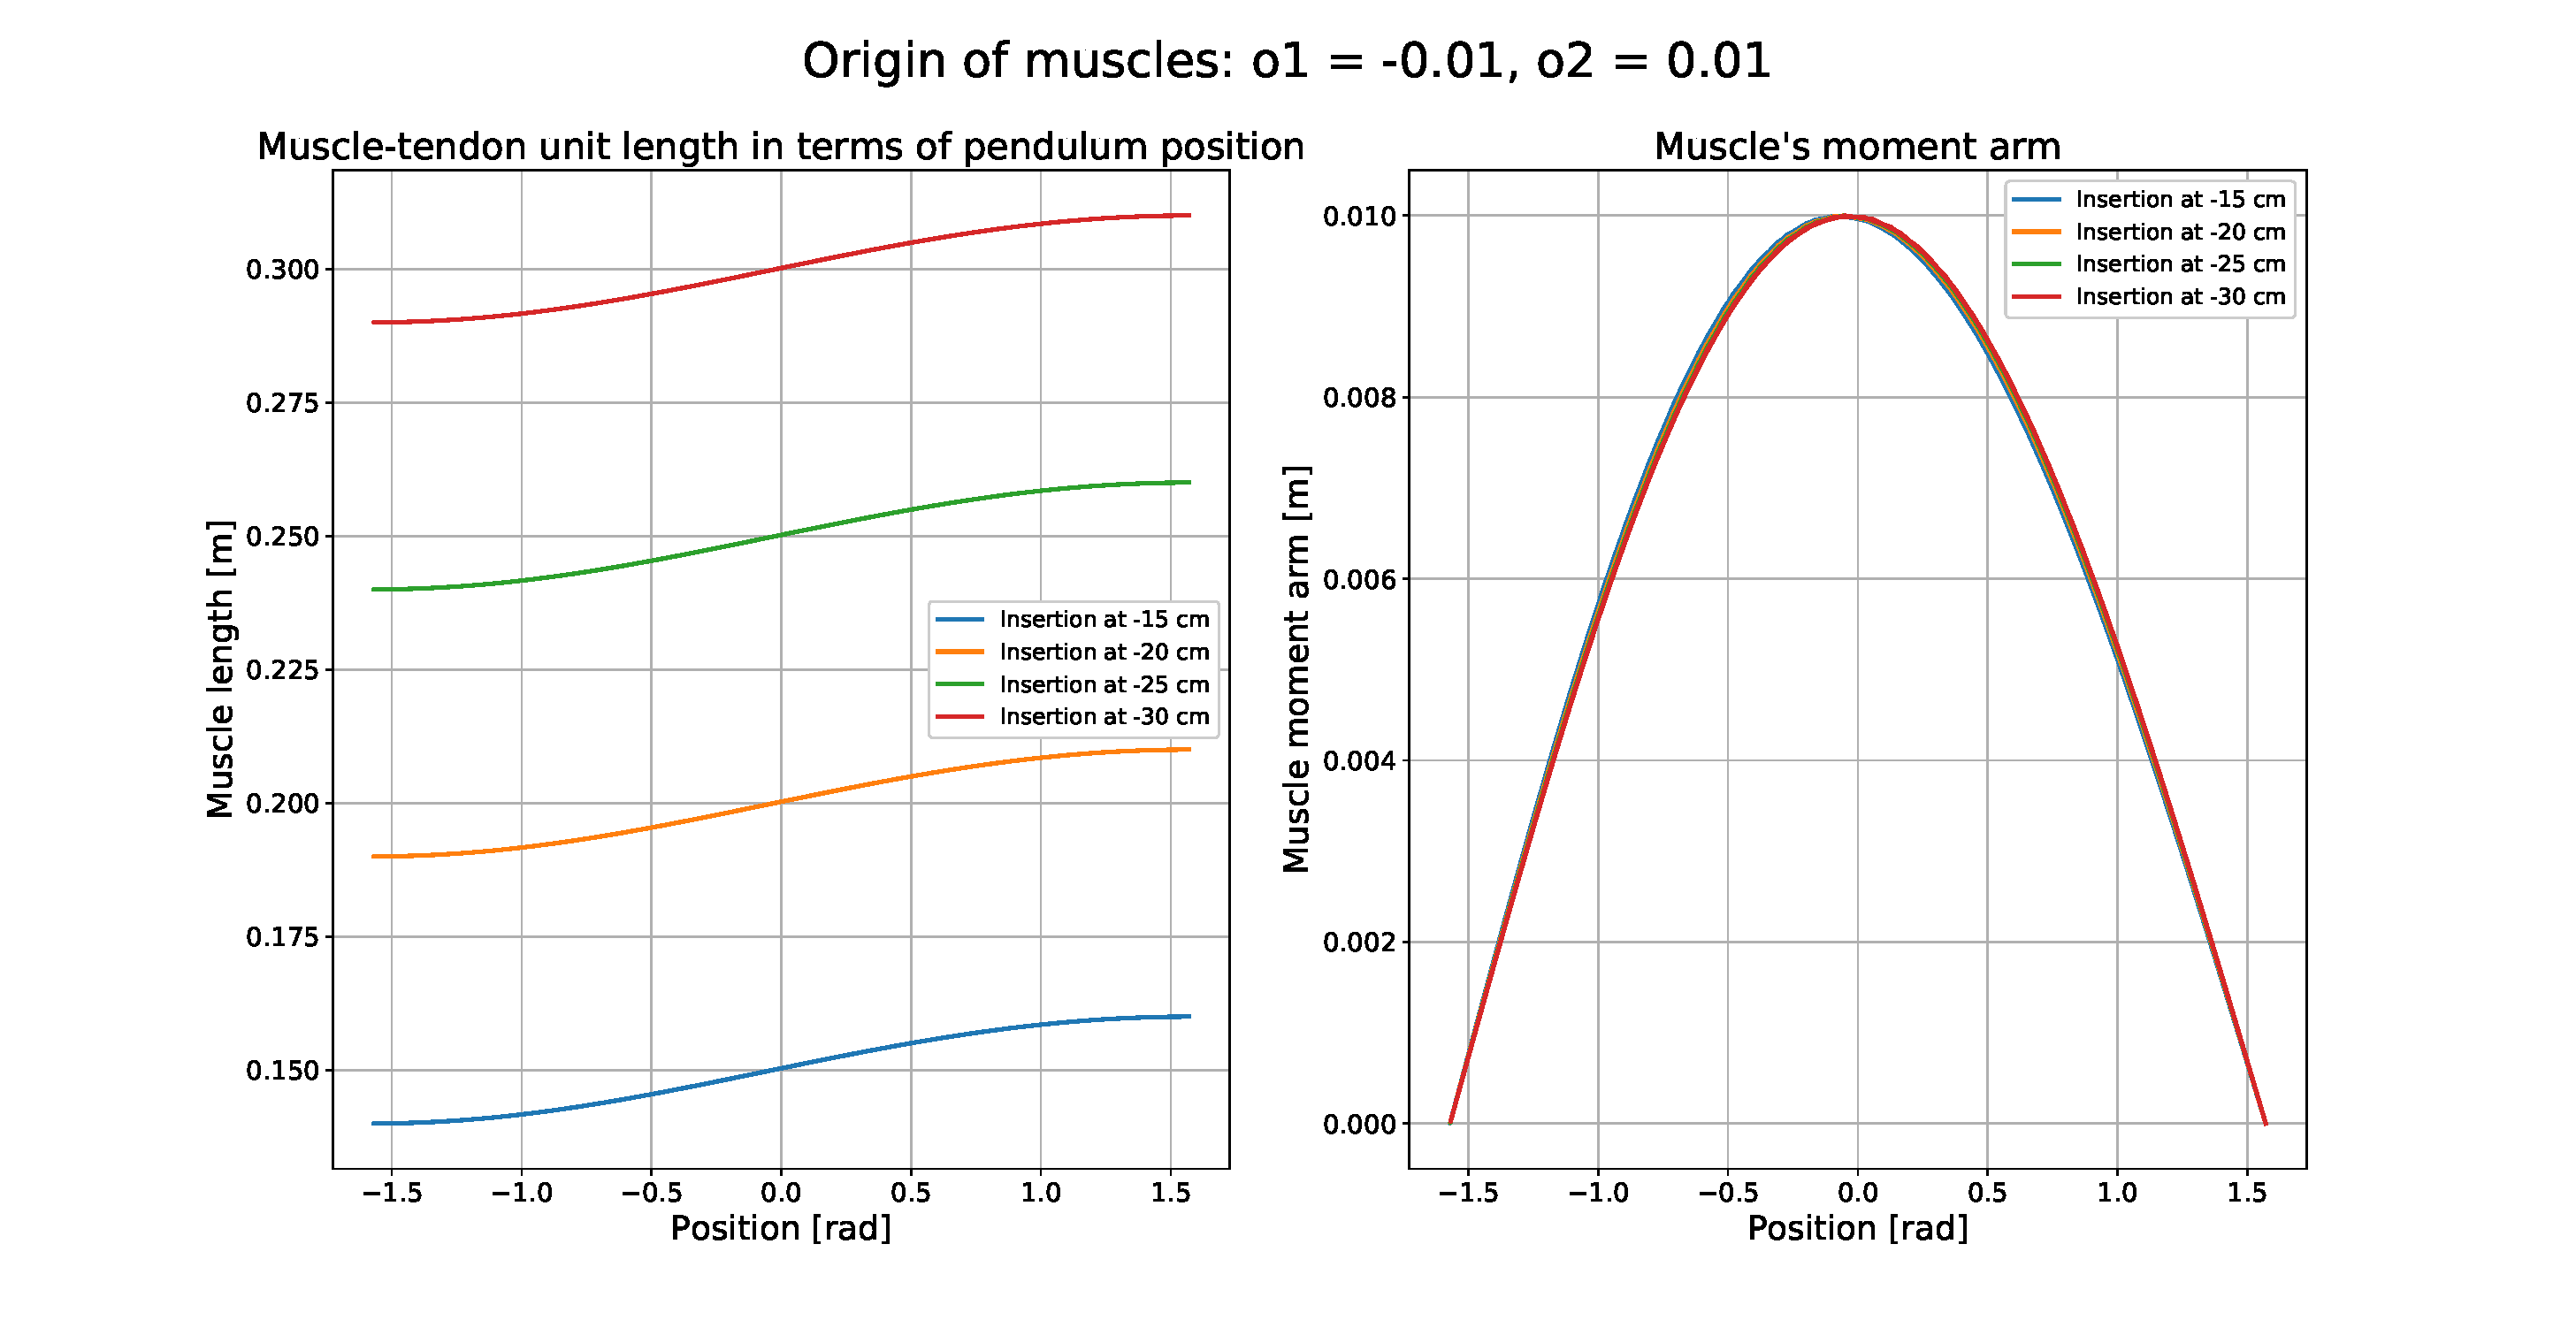
\includegraphics[width=1\textwidth]{o1_0_01.eps}%
  }\par\medskip
{
  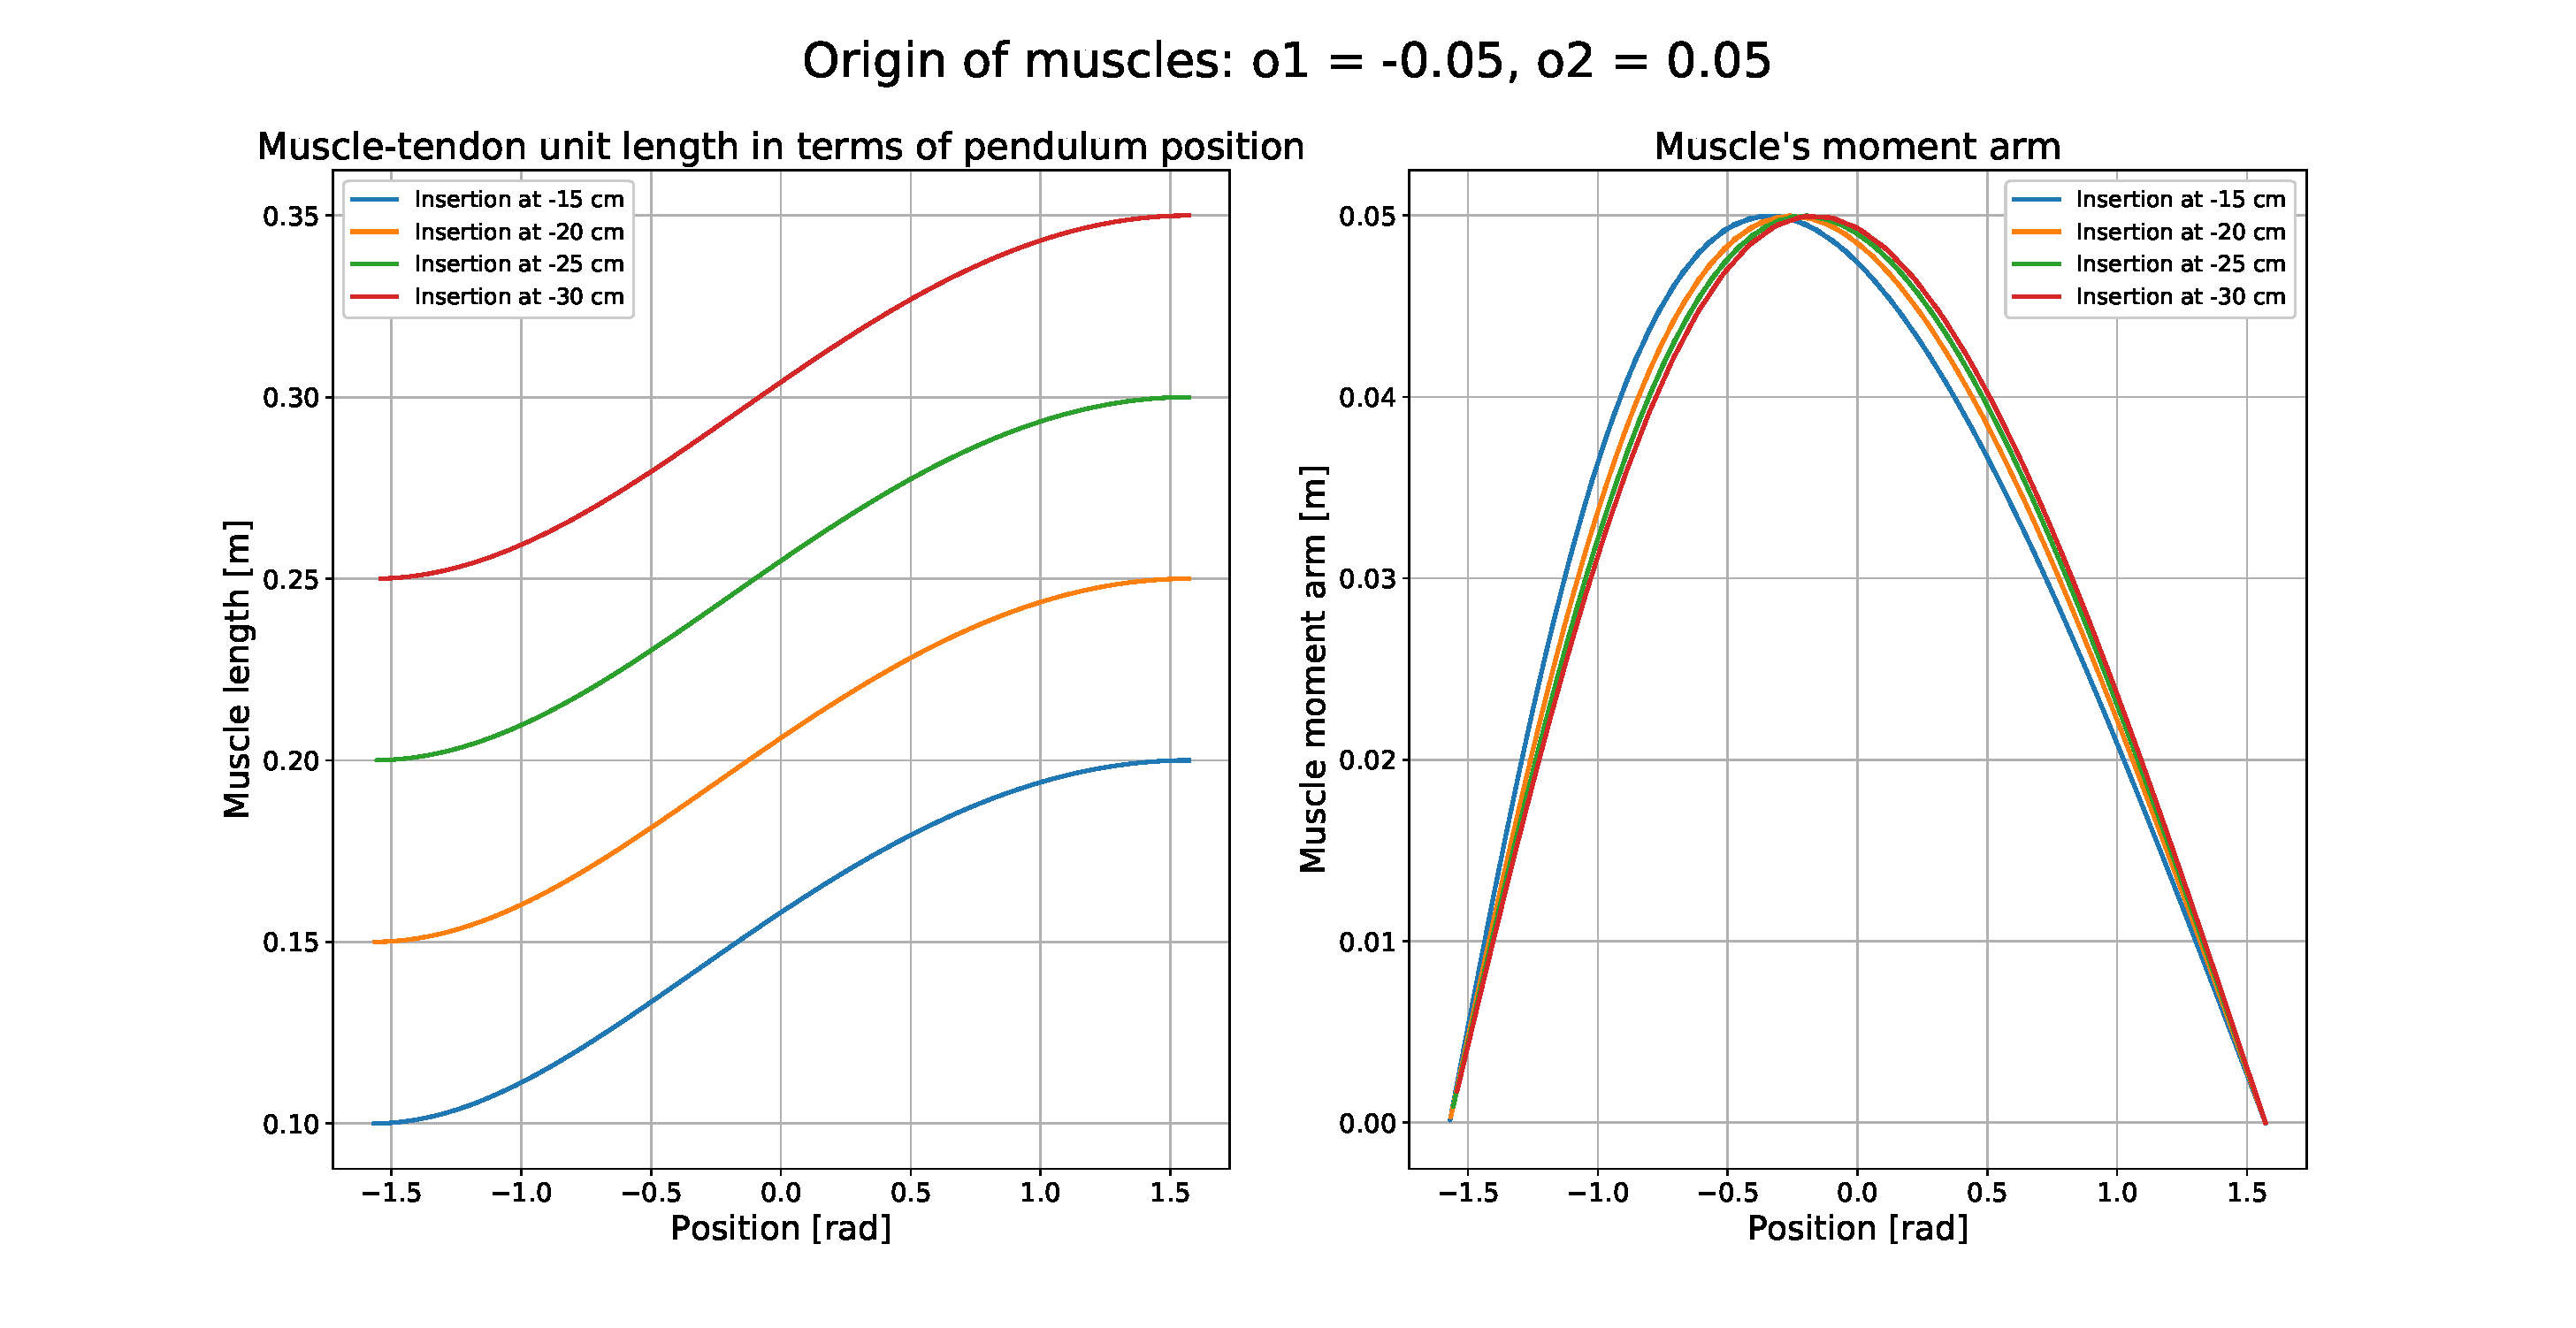
\includegraphics[width=1\textwidth]{o1_0_05.eps}%
  }  
\caption{Plot of muscle 1 length (\textbf{left}) and moment arm (\textbf{right}), with a varying insertion points -- the same for both $M1$ and $M2$ muscles. This figure continues with Figures \ref{figure:3a_1_follow} and \ref{figure:3a_1_end}. The muscles were active (activations = 0.05 throughout the simulation processes), the mass was set to 150 kg in order to cover the whole [$-\pi/2, \pi/2$] range and the simulation time was 5 sec.}
\label{figure:3_1a}
\end{figure}

\begin{figure} [H]
\centering
{%
  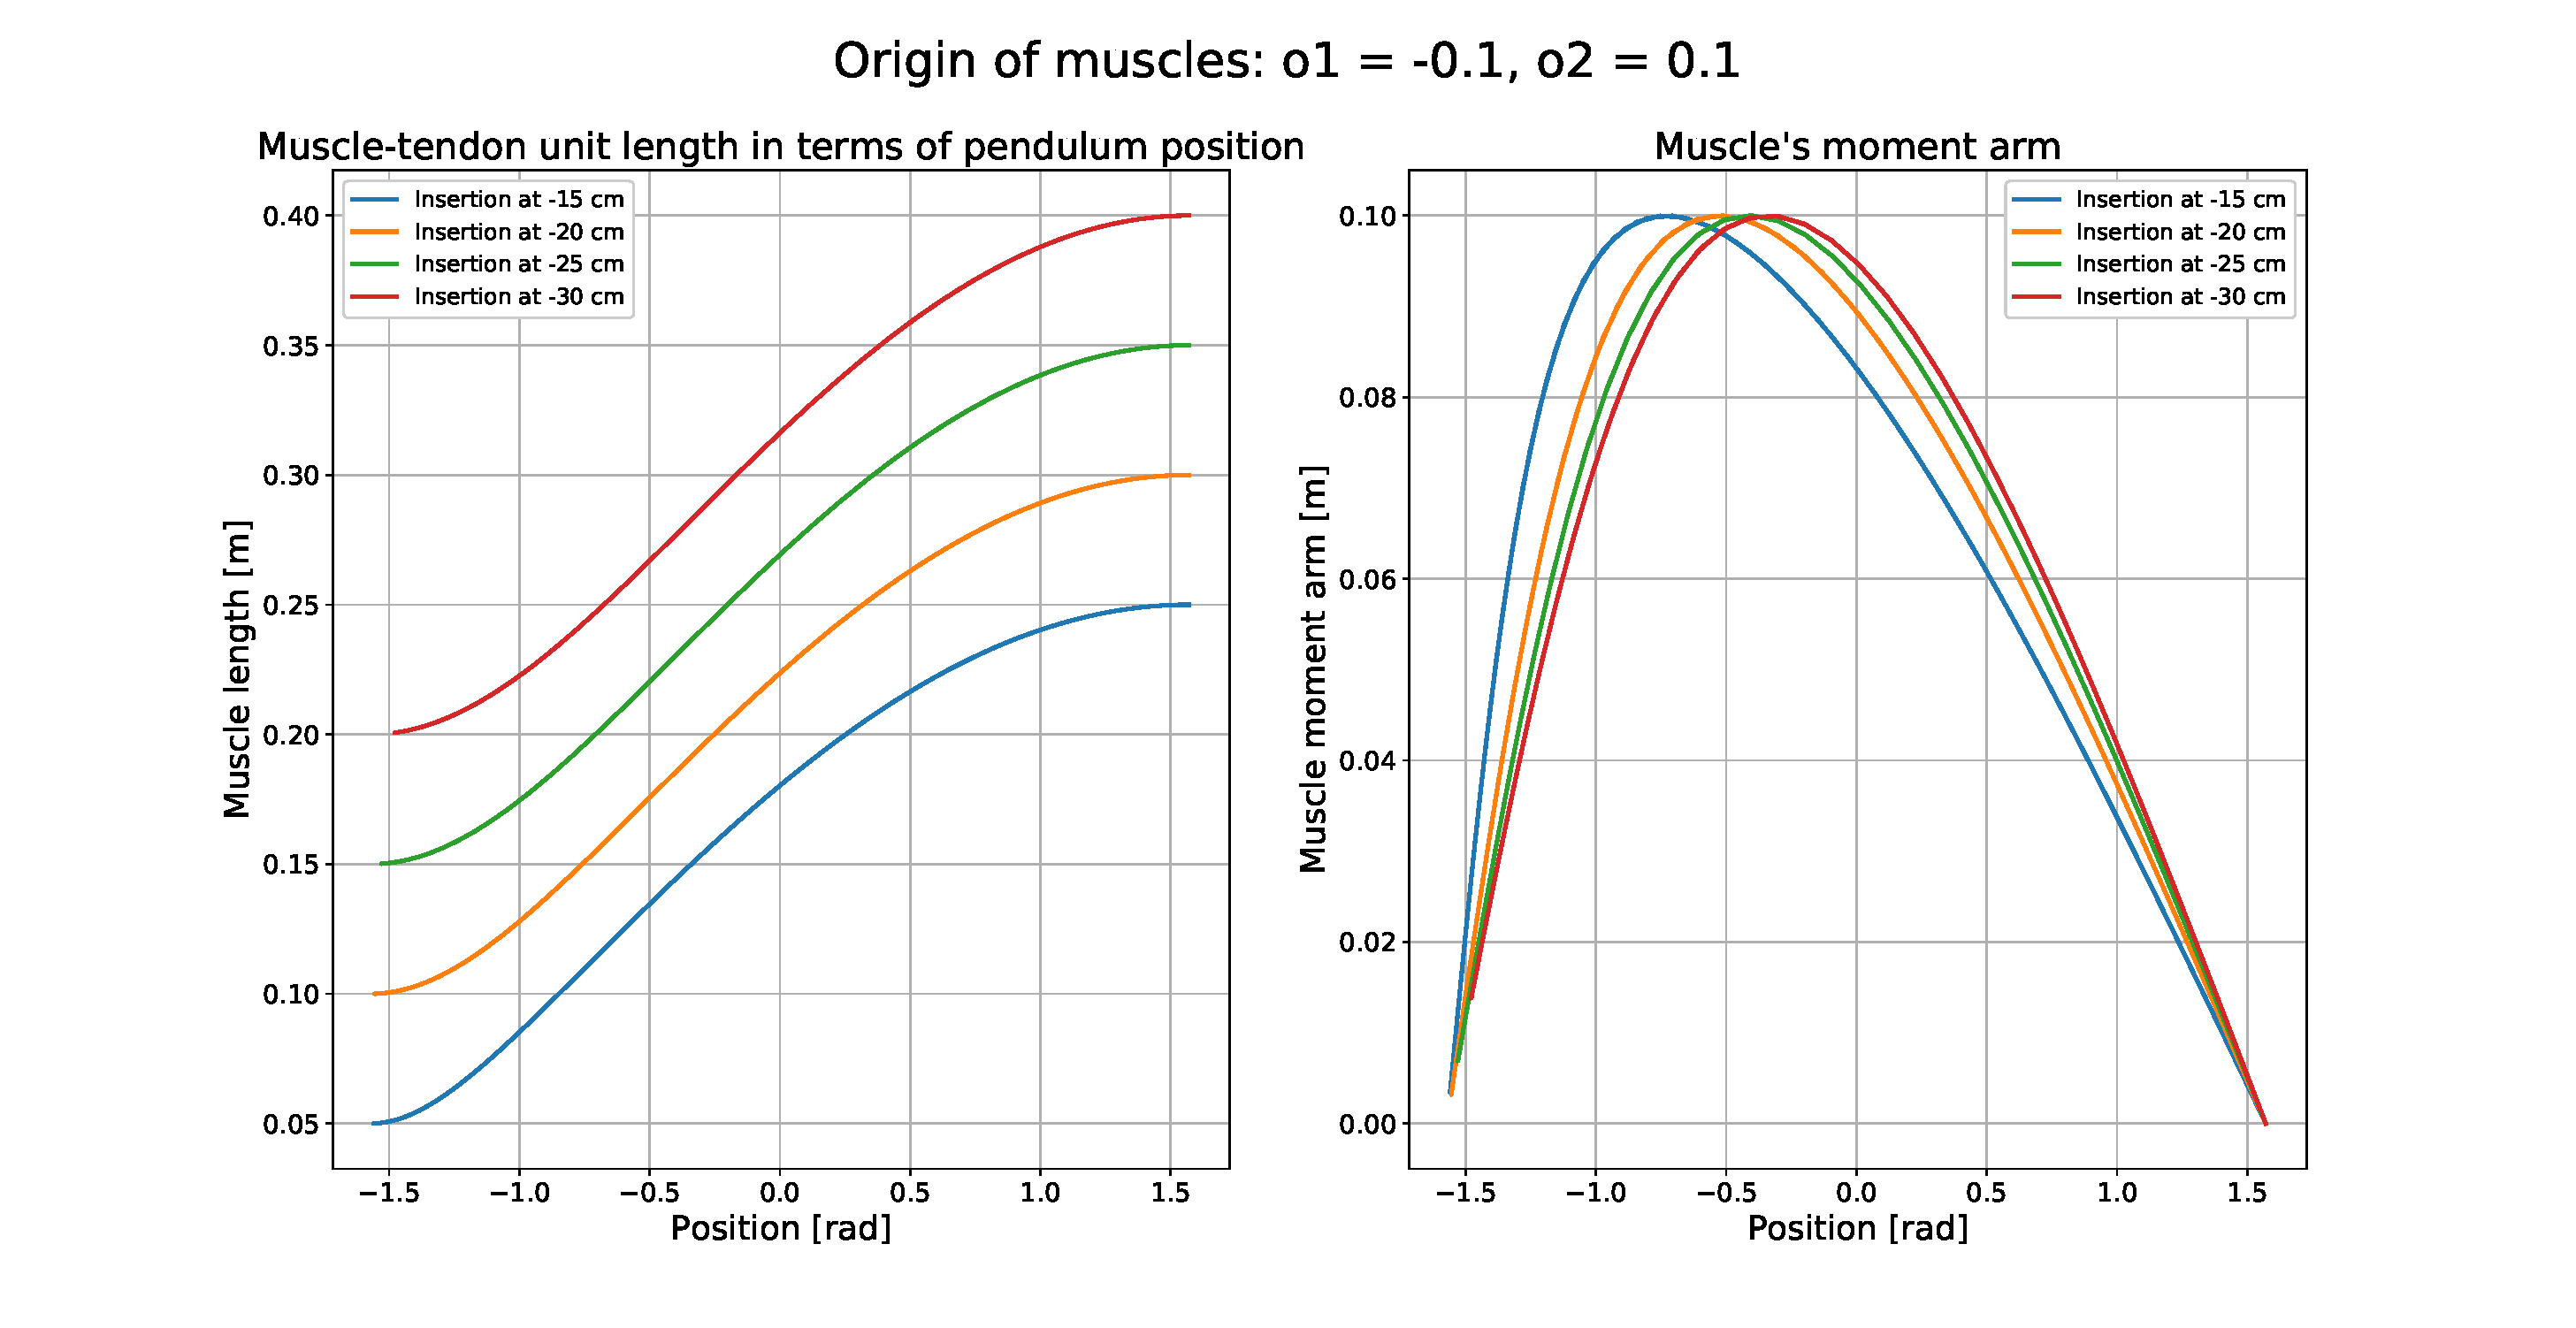
\includegraphics[width=1\textwidth]{o1_0_1.eps}%
  }\par\medskip
{%
  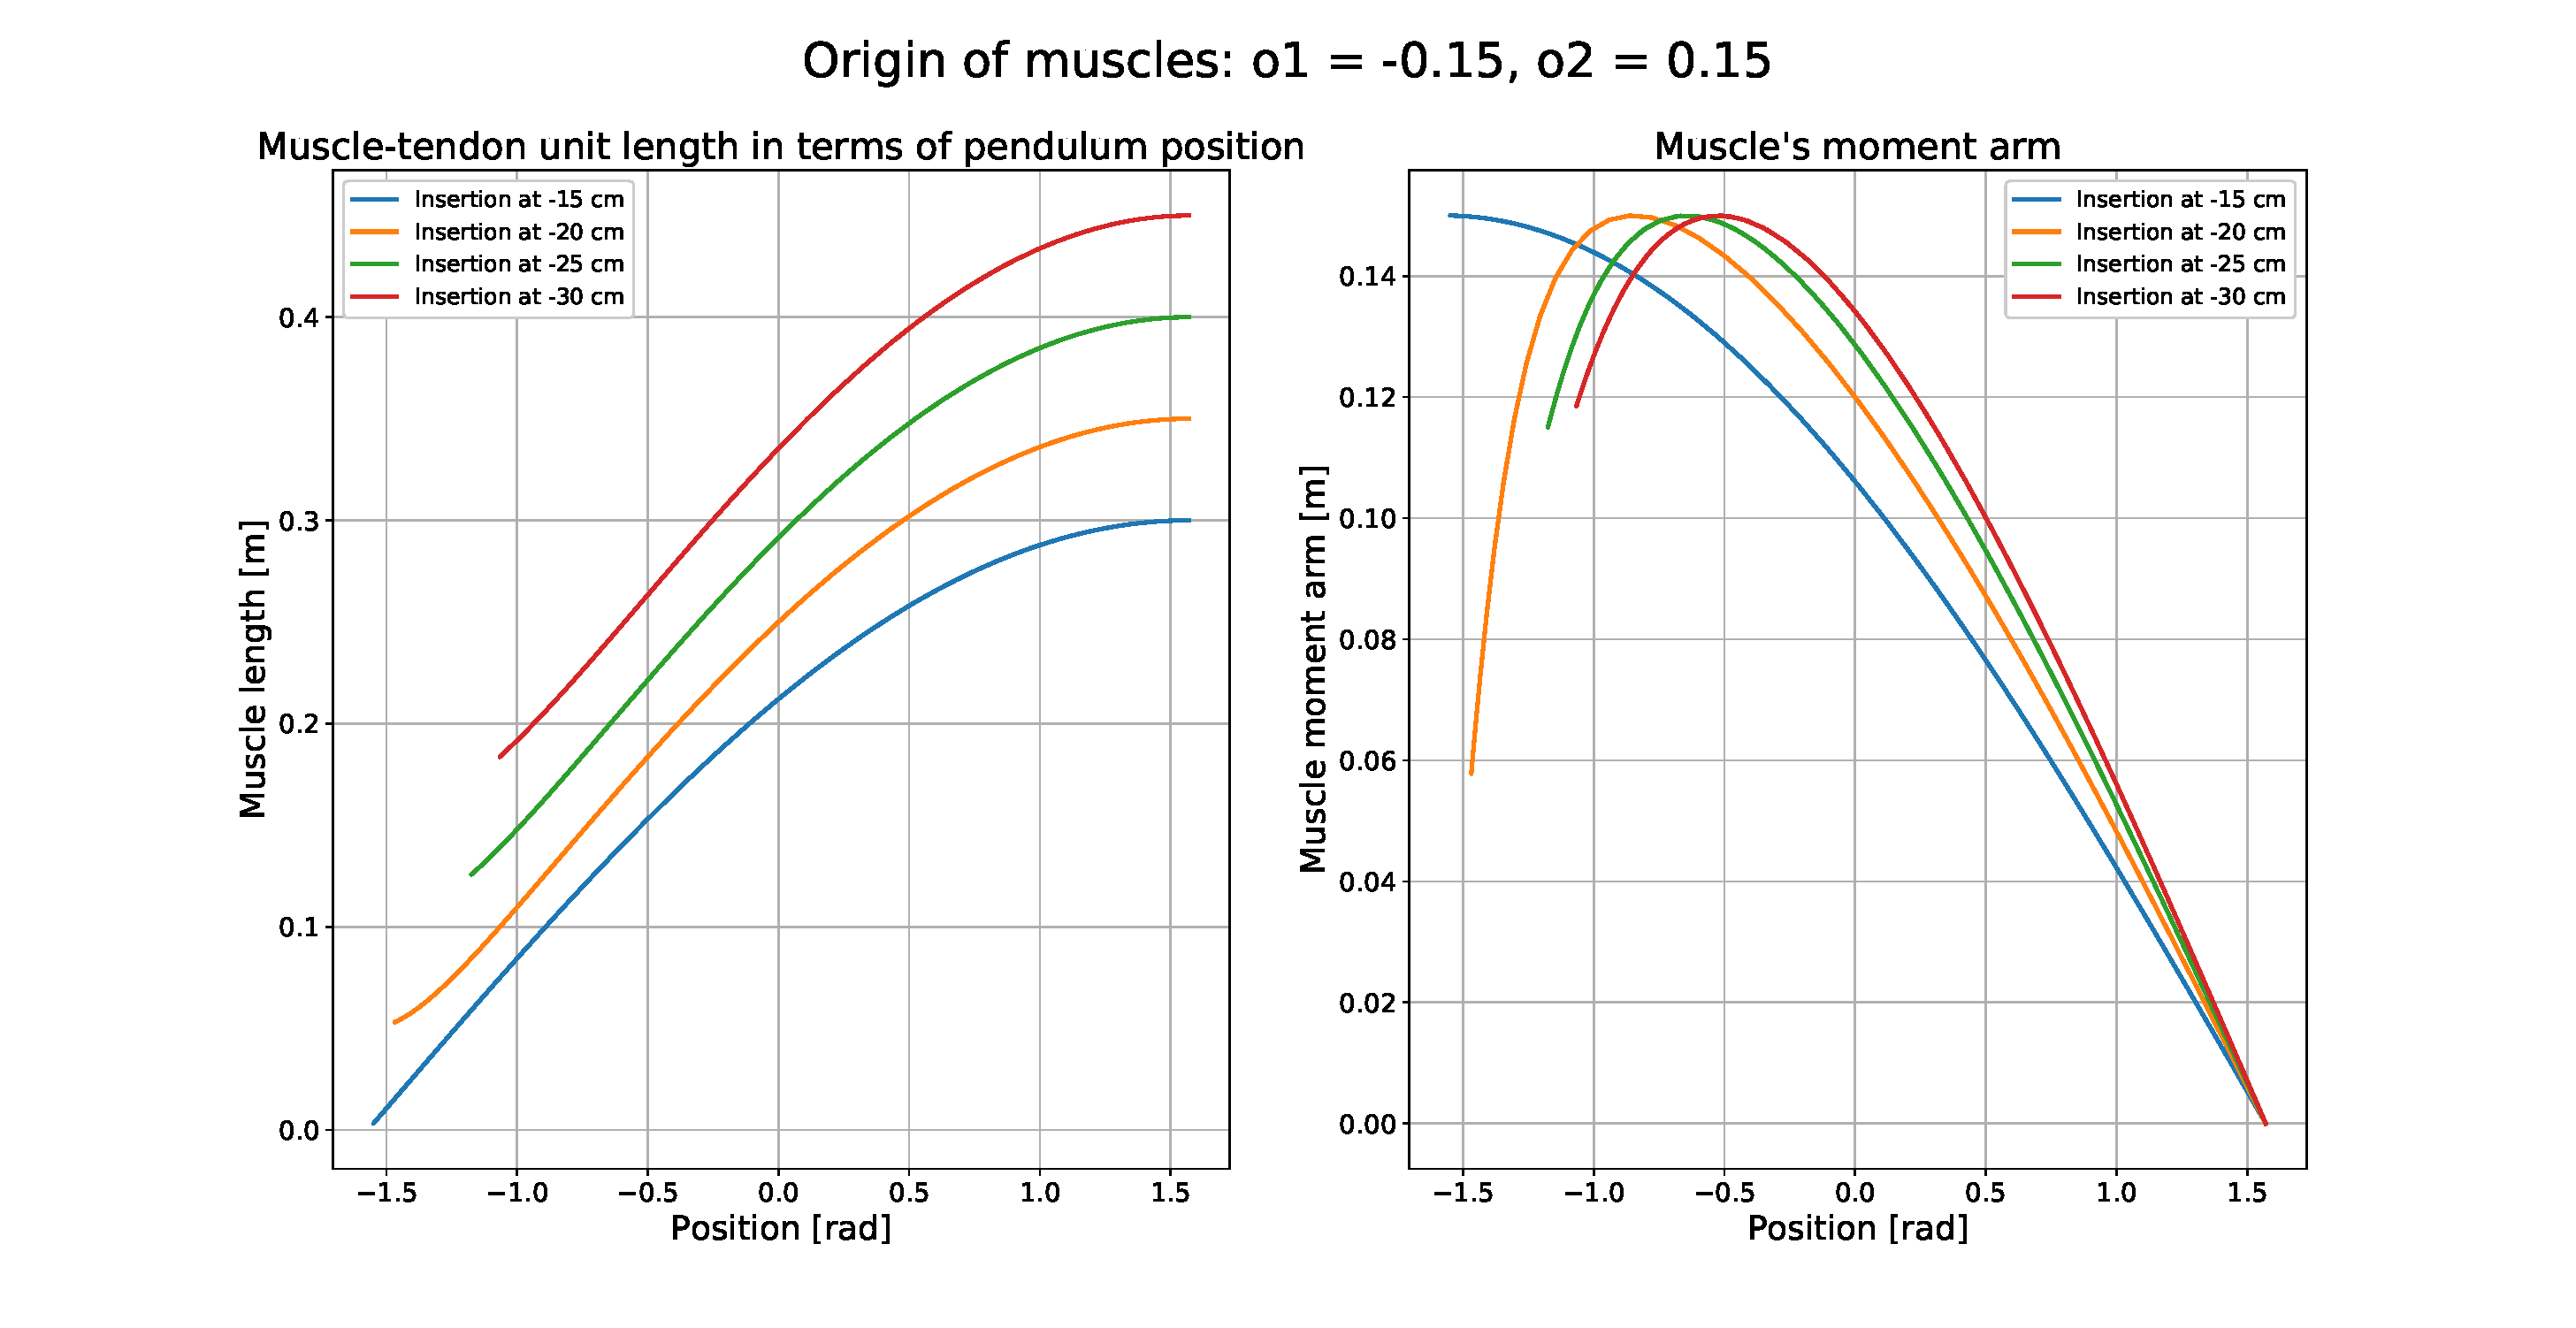
\includegraphics[width=1\textwidth]{o1_0_15.eps}%
}
\caption{Following of Figure \ref{figure:3_1a}}
\label{figure:3a_1_follow}
\end{figure}

\begin{figure} [H]
\centering
{%
  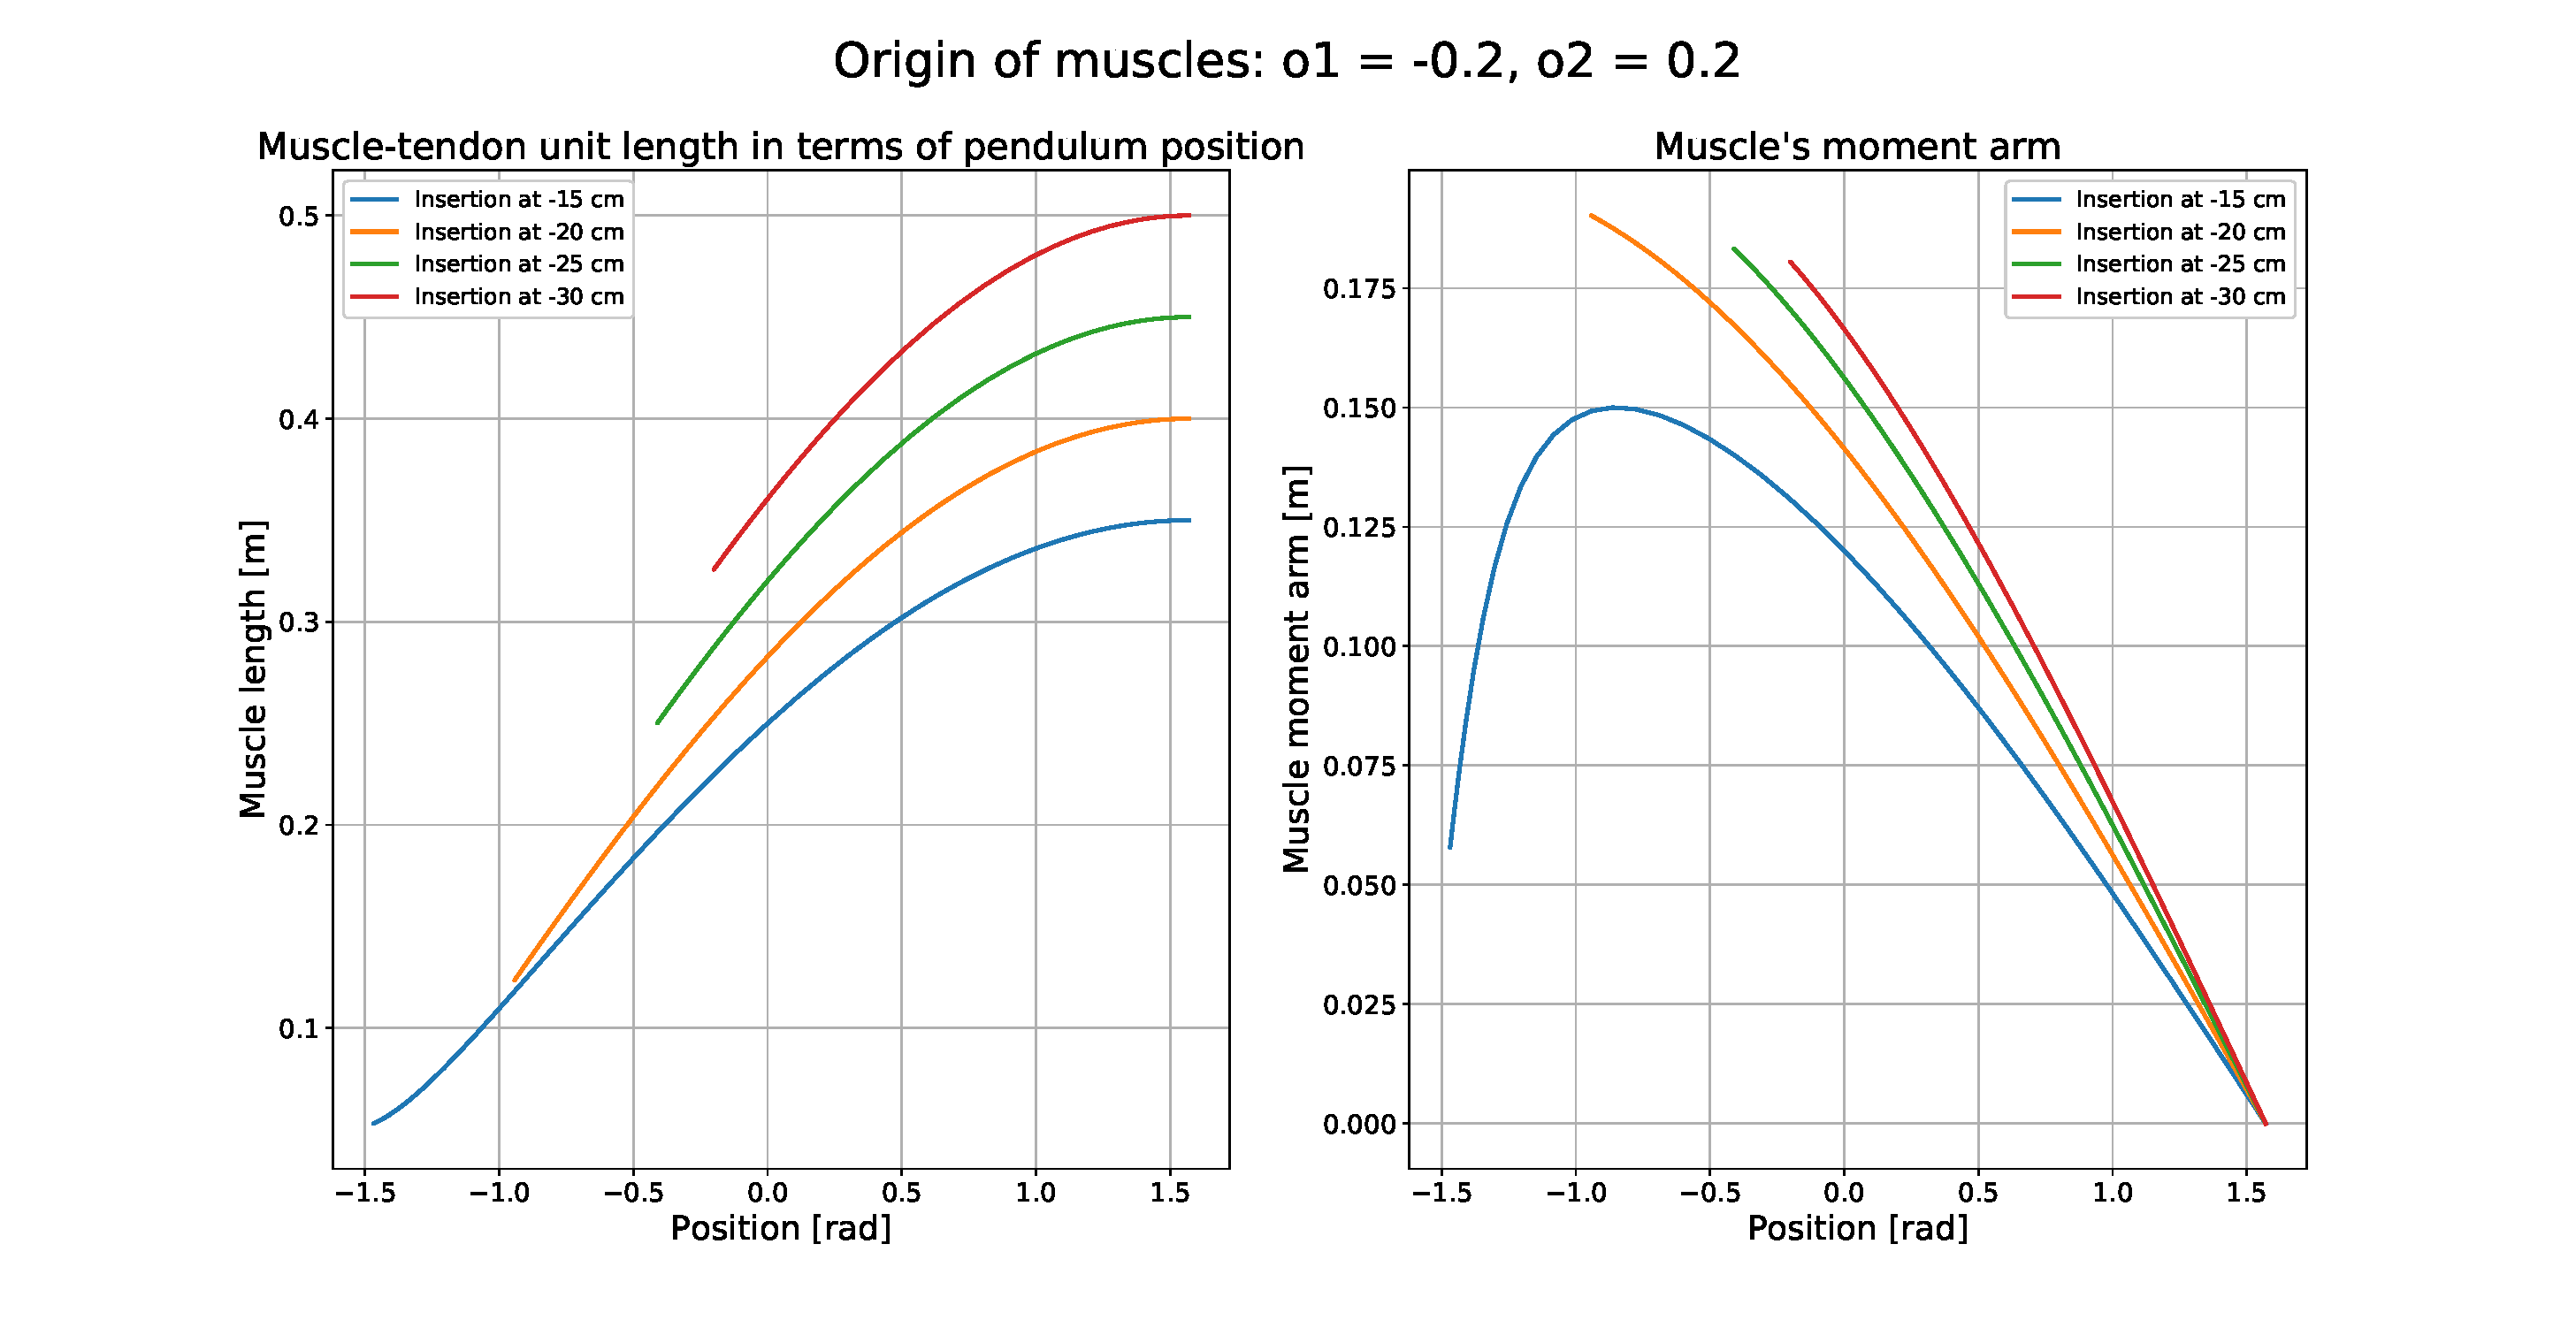
\includegraphics[width=1\textwidth]{o1_0_2.eps}%
  }
\caption{Following and end of Figures \ref{figure:3_1a} and \ref{figure:3a_1_follow}}
\label{figure:3a_1_end}
\end{figure}

\subsection*{3b. Under passive conditions (muscle is not activated),
  Discuss the effect of muscle attachment points on the pendulum's
  behavior. You can use the results from previous question to support
  and explain the pendulum's behavior.}
\label{sec:3b}

To assess the effects of muscles inactivation on the system -- that is -- purely passive conditions, we set the muscles origins for $M1$ and $M2$ at 17 cm from the pivot point and set $M1$'s and $M2$'s insertions at 5 cm and 20 cm respectively down the pivot point on the pendulum, in order not to have an equilibrium point of 0.0 rad. The mass used was 100 kg and the simulation time 10 seconds. We also repeated the simulation of point 3a under passive conditions.

Figure \ref{figure:HH} shows that the moment arms under passive conditions (right) do not change their dynamics as compared to the active setup (left). As a matter of fact, the muscle lengths dynamics are the same for both conditions (data not shown). What we can understand finally is that the intrinsic geometrical properties of the muscles -- lengths and arms -- do not depend on an activated or passive setup. Concerning the moment arms, we observe that, for a given origin (0.1 meters apart from the pivot point for both muscles), a lower insertion (e.g. 30 cm down the pivot point) will cause the max of the muscle torque to be closer to the 0.0 rad position, which can be more useful for this muscle to "call back" the pendulum towards him when it approaches the 0.0 rad position form the other side. All in all, we can appreciate the pendulum's equilibrium position with the moment arms, since both $M1$'s and $M2$'s torques must be equal in order to achieve equilibrium -- of course, gravity has its say in the matter, as we can observe in the next result:

Figure \ref{figure:activepassive} shows distinct behaviors with and without activation of muscles, in the evolution of the system position as a function of time. The passive system takes more time to stabilize and lay closer to 0 rad, compared to the activated system setup. Activation of muscle acts as dampeners, facilitating stabilization which occurs faster time-wise. Passive muscles have a smaller momentum due to the fact that they don't generate an active force; the pendulum in passive setup is then more influenced by gravity and rests at a smaller angle with respect to the 0.0 rad position.

\begin{figure}[ht!]
    \centering
    \begin{subfigure}[t]{0.5\textwidth}
        \centering
        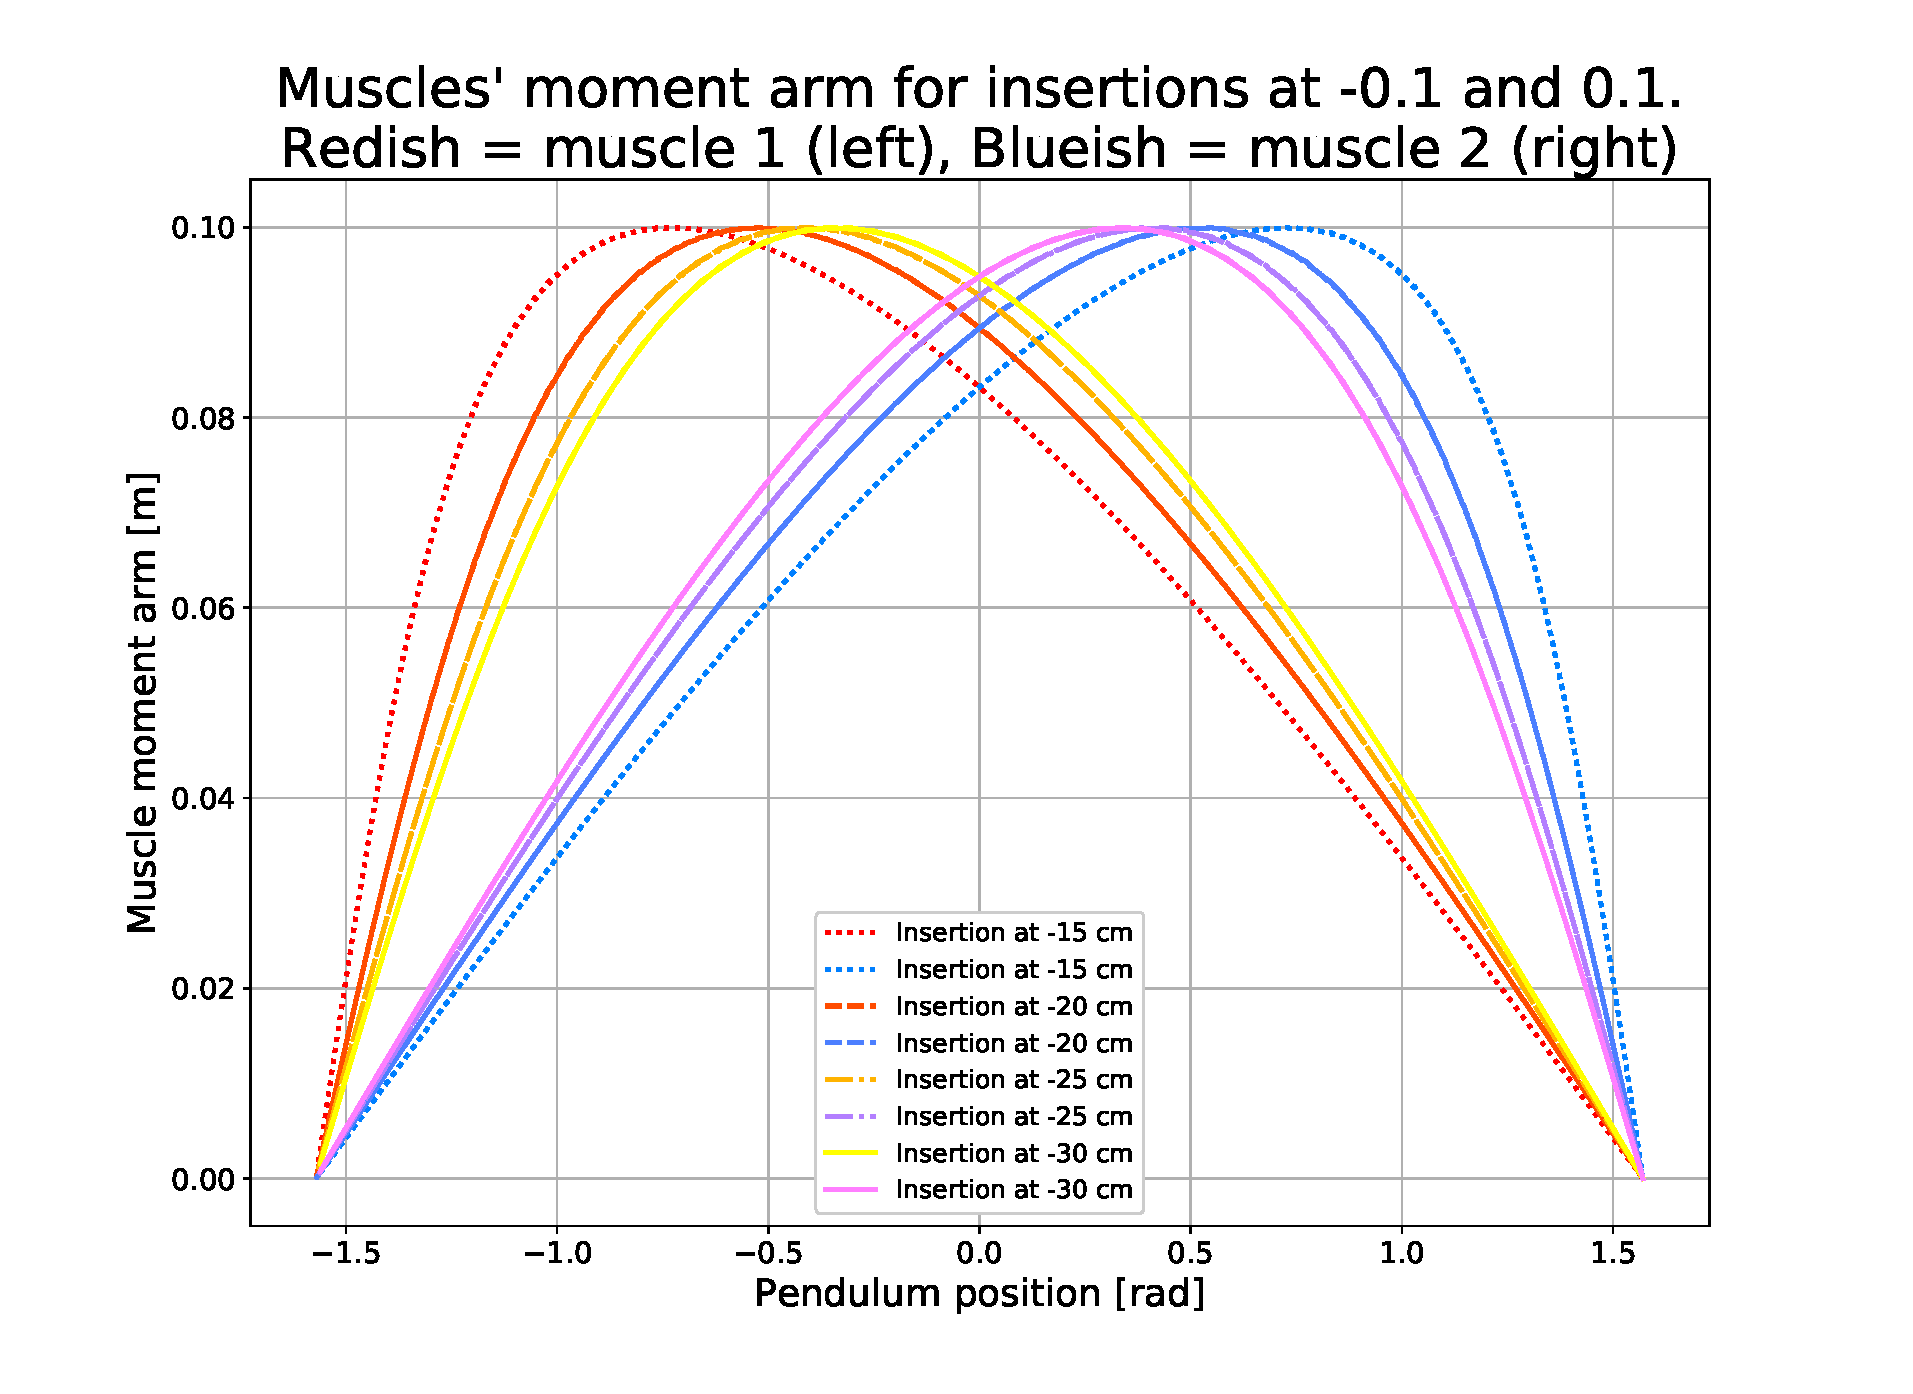
\includegraphics[height=2.5in]{HH_act.eps}
        \caption{}
    \end{subfigure}%
    ~ 
    \begin{subfigure}[t]{0.5\textwidth}
        \centering
        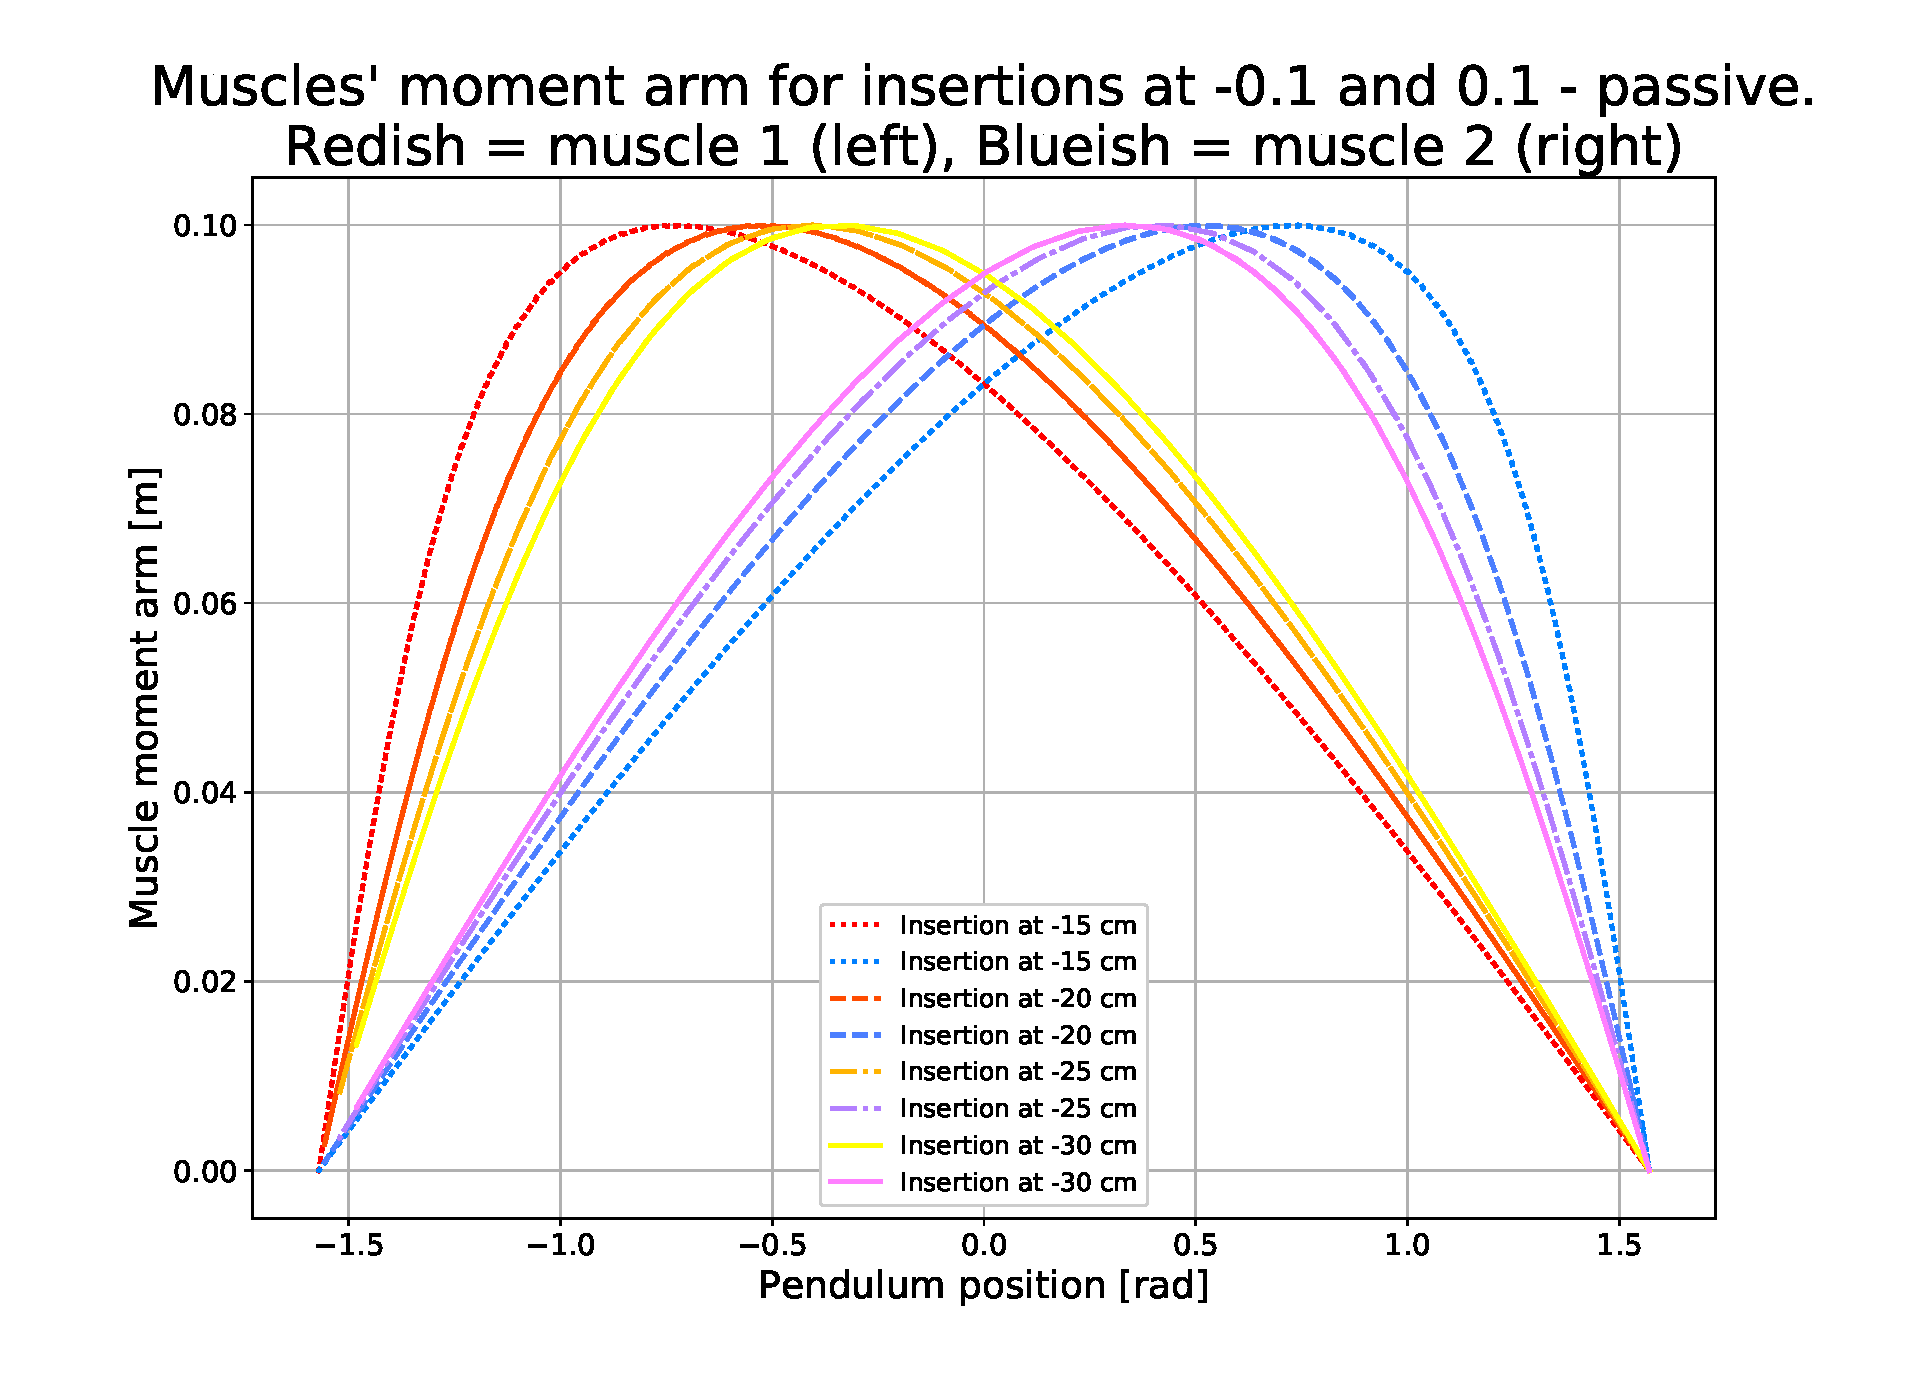
\includegraphics[height=2.5in]{HH_pass.eps}
        \caption{}
    \end{subfigure}
    \caption{Muscle moment arm size as a function of pendulum position. (a) Representation for an active (activation=0.25) muscle simulation. (b) Representation for a passive muscle simulation. Both (a) and (b) looks identical.}
    \label{figure:HH}
\end{figure}

\begin{figure}[ht!]
    \centering
    \begin{subfigure}[t]{0.5\textwidth}
        \centering
        \includegraphics[height=2.5in]{Active.eps}
        \caption{}
    \end{subfigure}%
    ~ 
    \begin{subfigure}[t]{0.5\textwidth}
        \centering
        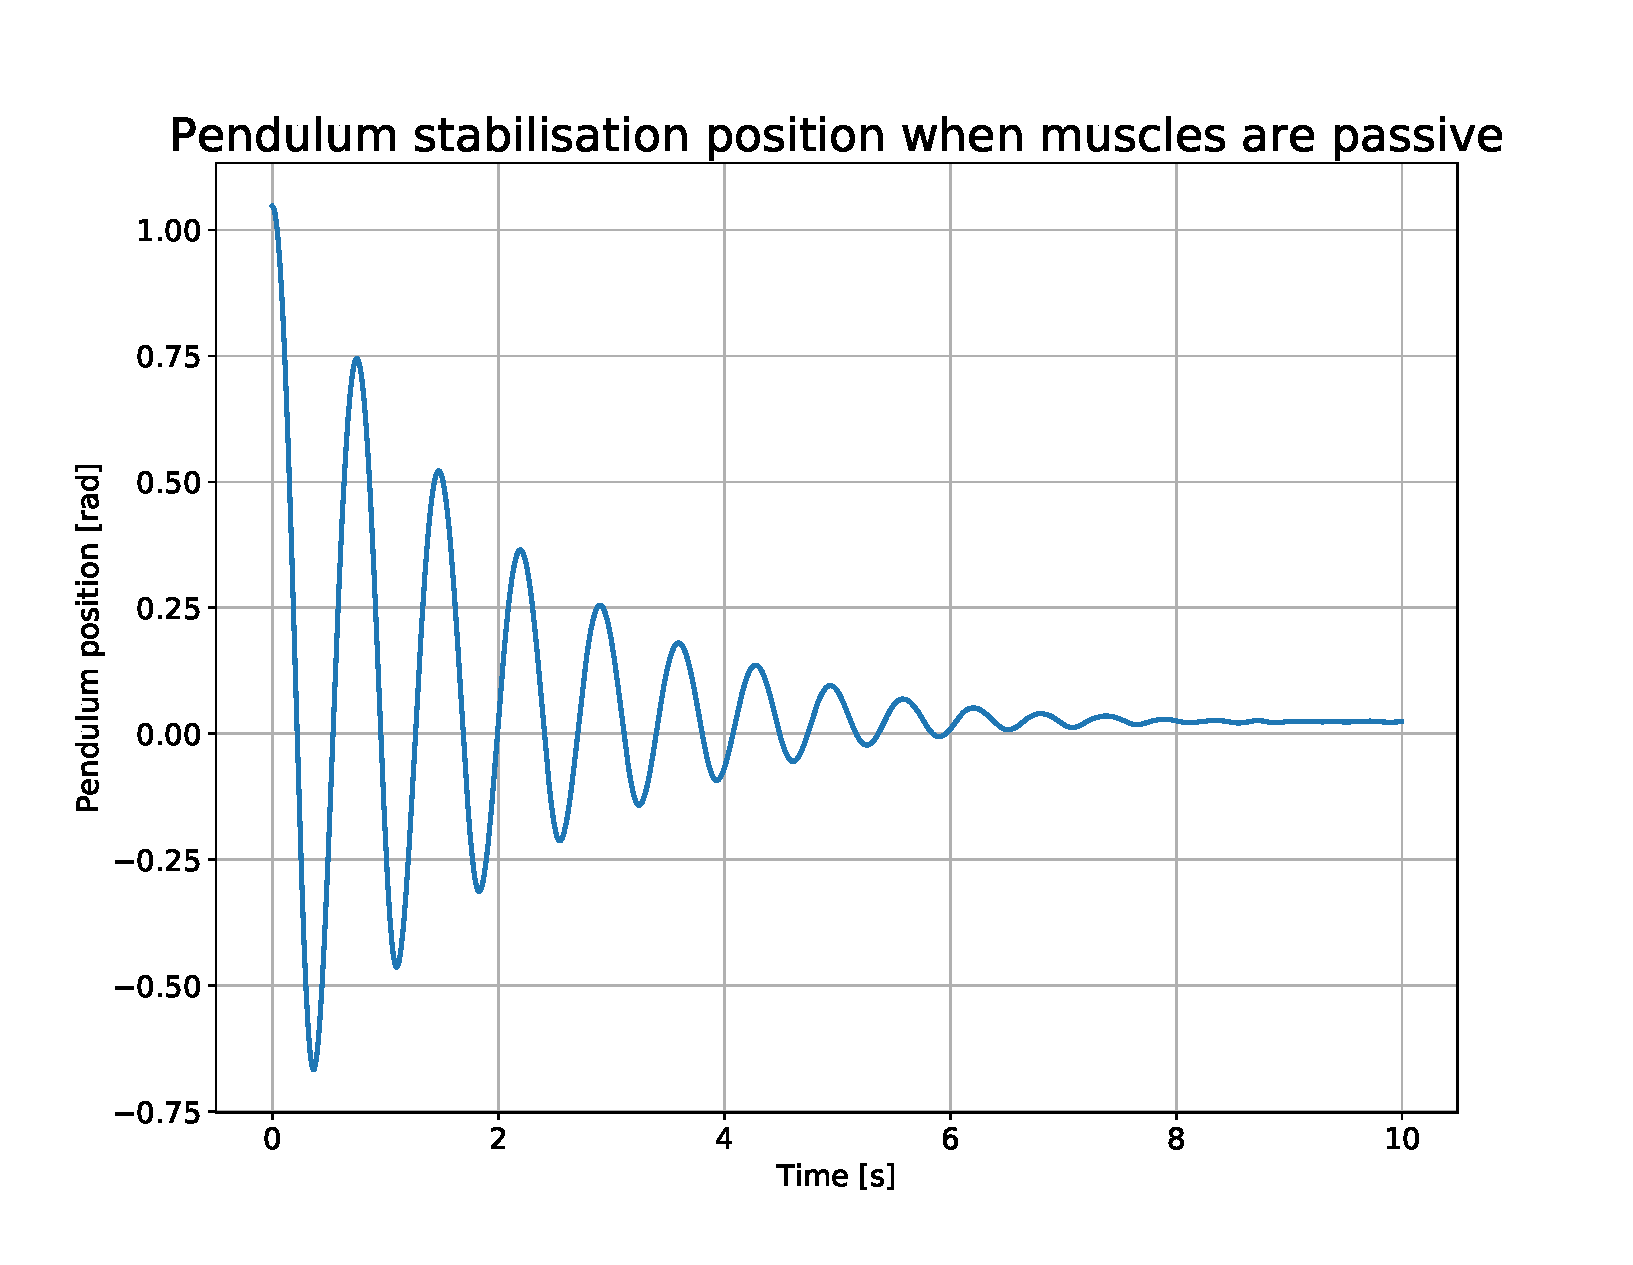
\includegraphics[height=2.5in]{Passive.eps}
        \caption{}
    \end{subfigure}
    \caption{Pendulum position as a function of time. (a) Stabilization of pendulum with an active (activation=0.25) muscle simulation. (b) Stabilization of pendulum with a passive muscle simulation. Passive muscle stabilizes slower and closer to 0 rad, compared to the active muscle case. The following parameters where used: mass=100kg, origin=0.17, insertion1=0.05, insertion2=0.2.}
    \label{figure:activepassive}
\end{figure}

\clearpage
\subsection*{3c. Using simple activation wave forms (example : sine or
  square waves) applied to muscles (use
  \fileref{SystemSimulation.py::add\_muscle\_activations} method in
  \fileref{exercise3.py}), try to obtain a limit cycle behavior for
  the pendulum. Use relevant plots to prove the limit cycle behavior.
  Explain and show the activations wave forms you used. If needed, use
  \fileref{PendulumSystem.py::Pendulum::derivative} function to
  perturb the model.}
\label{sec:3c}

Using a sinusoidal activation pattern -- displayed in Figure \ref{fig:acts} -- we obtained a fast limit cycle behavior, as shown in Figure \ref{figure:3c}, where (a) shows the limit cycle and (b) shows that after a perturbation -- which consisted in suddenly force the pendulum's position to 1 rad -- the pendulum gets back to the same trajectory as before. The phase portraits were consistent with a limit cycle behavior (data not shown). A video of the simulation is available at \url{https://www.youtube.com/watch?v=W5Ozosefc9c}. 

\begin{figure}[ht!]
    \centering
    \begin{subfigure}[t]{0.5\textwidth}
        \centering
        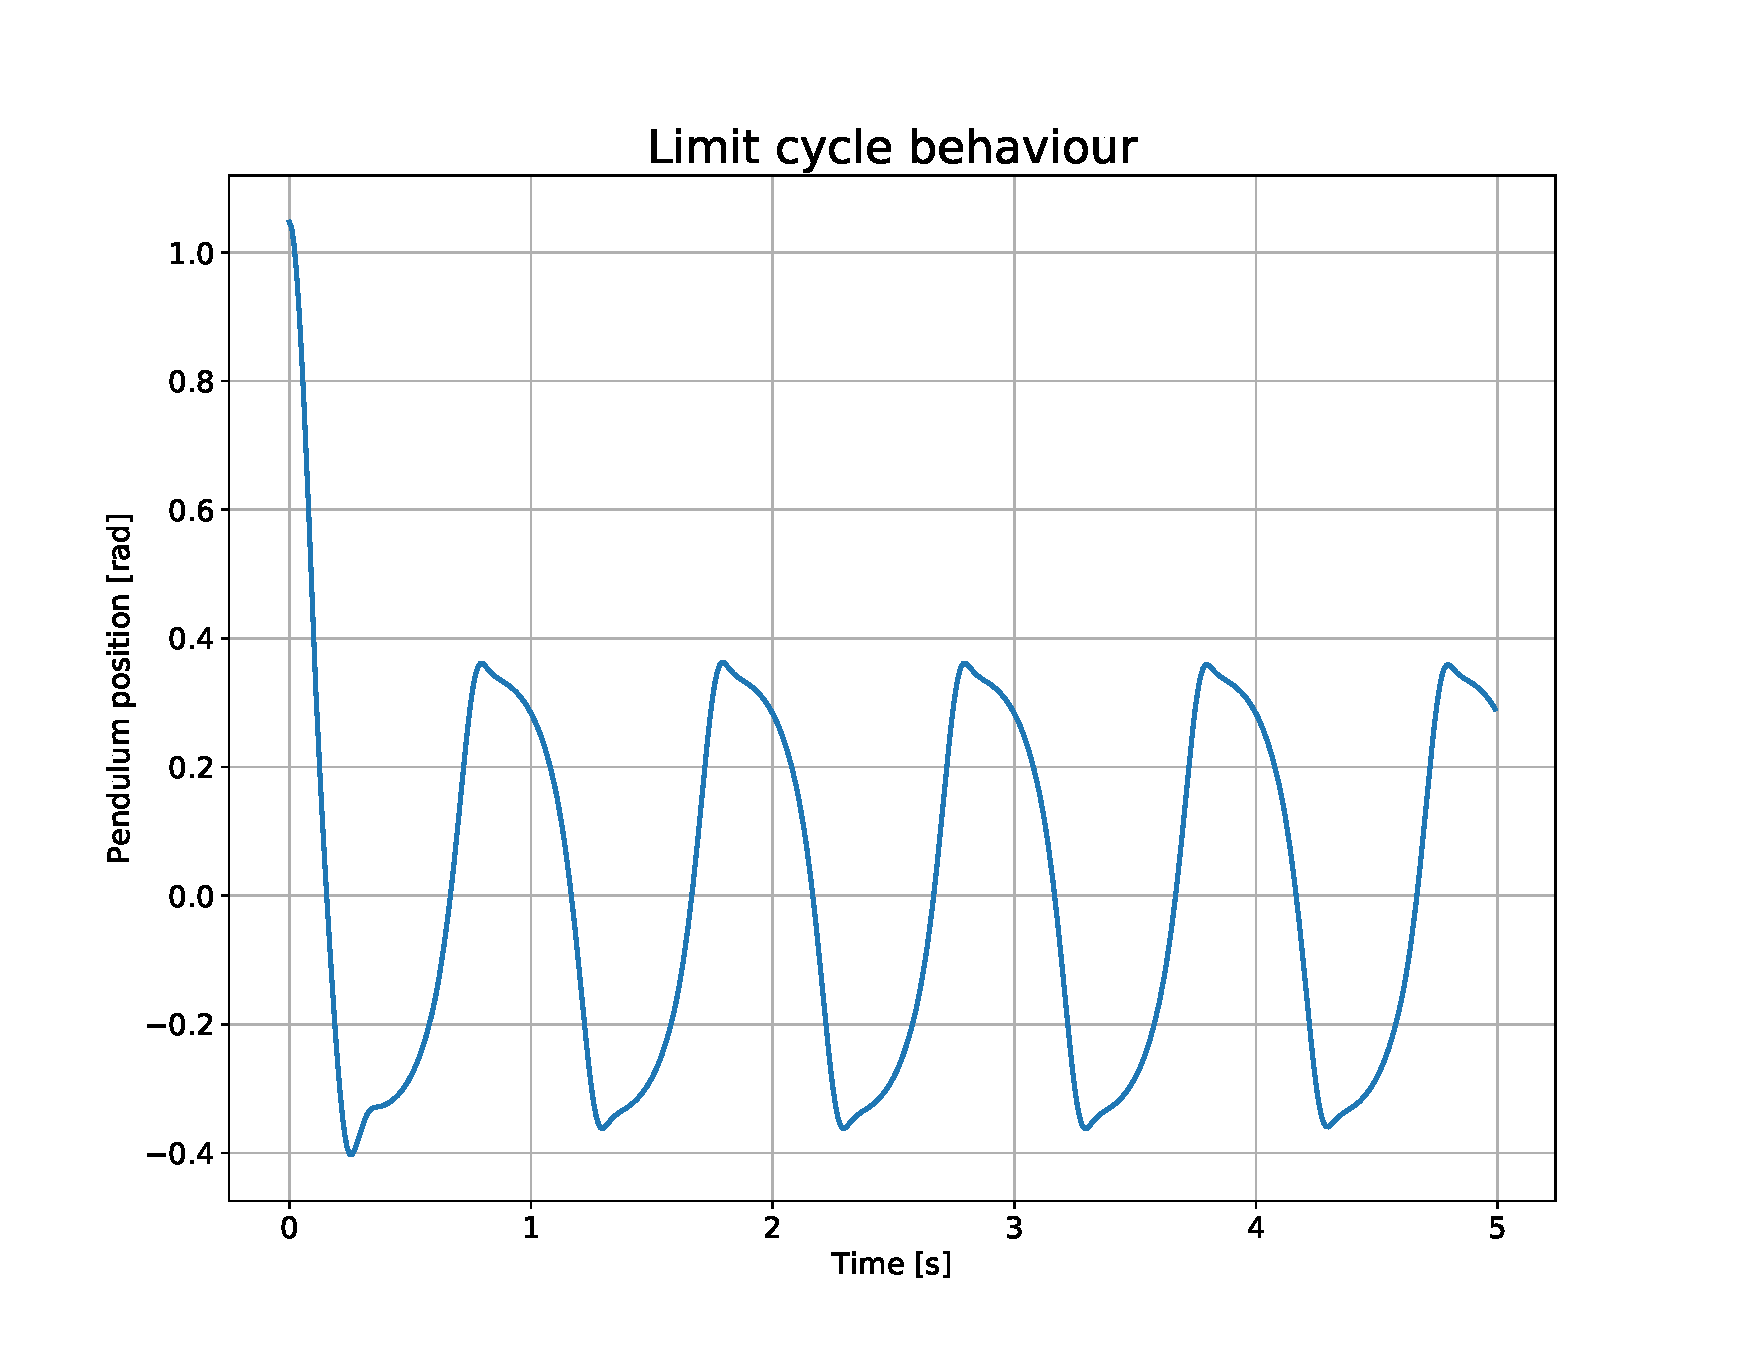
\includegraphics[height=2.5in]{LimitCycle.eps}
        \caption{}
    \end{subfigure}%
    ~ 
    \begin{subfigure}[t]{0.5\textwidth}
        \centering
        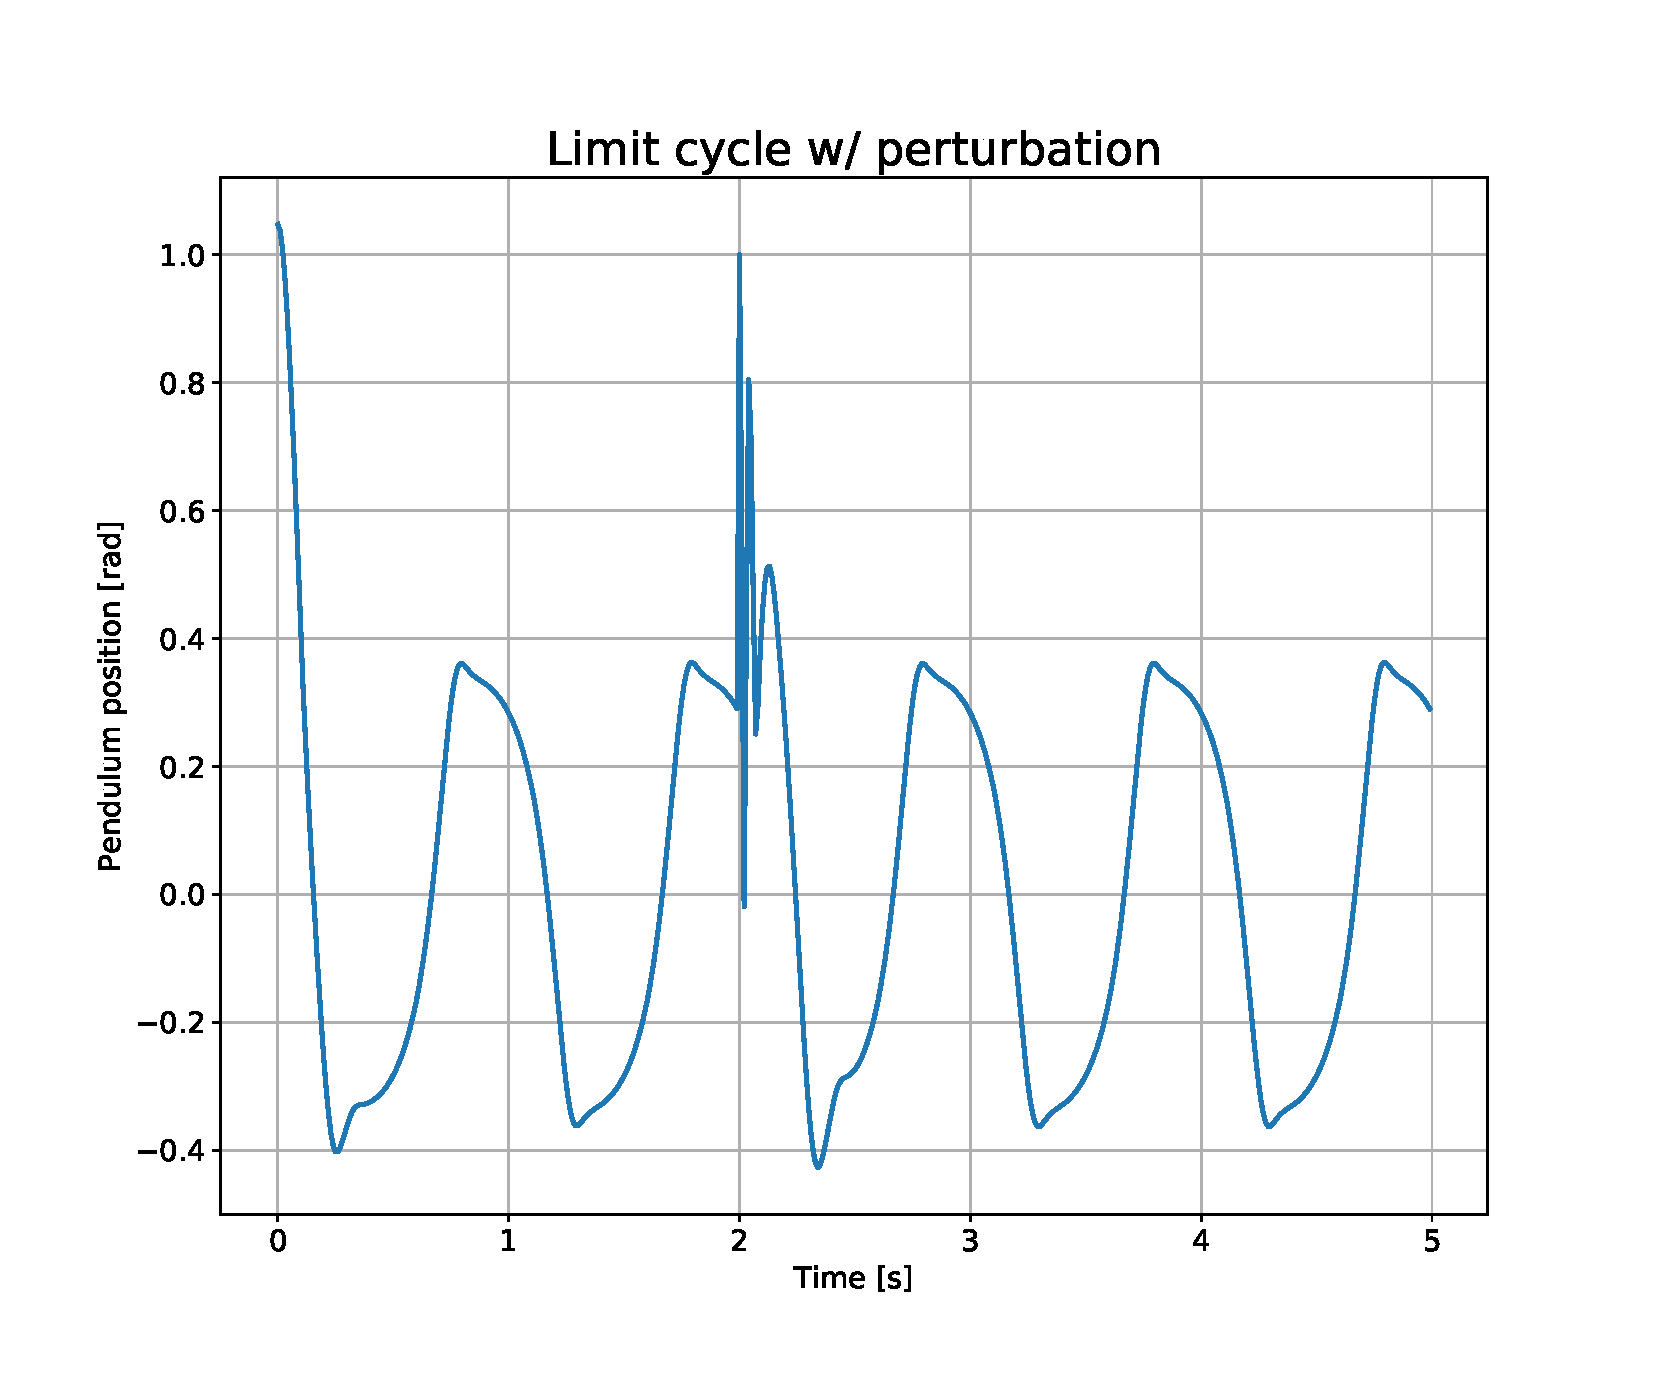
\includegraphics[height=2.5in]{LimitCyclePertu.eps}
        \caption{}
    \end{subfigure}
    \caption{ (a) Limit cycle behaviour of the pendulum. (b) After a small perturbation (forcing the pendulum's position to 1 rad) at time = 2 s, the pendulum goes back to the same behaviour as before, corroborating a limit cycle behaviour. Mass = 10 kg, activations are sinusoidal (see Figure \ref{fig:acts}). A video of this very stimulation is available at \url{https://www.youtube.com/watch?v=W5Ozosefc9c}.}
    \label{figure:3c}
\end{figure}

\begin{figure}[H]
  \centering
  \includegraphics[width=0.5\textwidth]{Activations.eps}
  \caption{Time-wise sinusoidal muscles activation.}
  \label{fig:acts}
\end{figure}

\subsection*{3d. Based on the previous limit cycle, show how the
  physical properties of the pendulum such as mass, length and inertia
  (Inertia is a result of mass and length) affect the amplitude and
  frequency of the pendulum oscillations for a given stimulation.}
\label{sec:3d}

The physics of this model tell us that there are two ways of playing with the pendulum's inertia: playing either with its mass or length. Simulating the same limit cycle as in 3c, we fixed the mass at 10 kg and plotted the pendulum's trajectory for a length of 0.5 m, which corresponds to the default pendulum's length, or 2 m -- see Figure \ref{figure:3d_1}. The left plot is the same as Figure \ref{figure:3c} (a), for the experimental settings are the same. However, Figure \ref{figure:3d_1} (b) shows that a longer pendulum, hence having a greater inertia, doesn't exhibit the same behavior: indeed, we observe that after the initial drop from the $\pi/2$ position, the first amplitude is higher than that of the 0.5 m pendulum, due to the grater inertia opposing the muscles dampening. Furthermore, the same greater inertia causes it to reach the limit cycle later than the 0.5 m pendulum, and to oscillate at a lower amplitude. This is due to the fact that since the pendulum has a greater inertia, the muscles' actions on it will have less effect -- as inertia is defined as a resistance against movement -- and the pendulum won't be pulled as strongly as when it measures 0.5 m. One will also notice that this greater inertia also acts as a "smoother", since the little irregularities in the trajectory's curve have disappeared. The limit cycle oscillatory frequency is, however, unchanged (1 Hz).  


\begin{figure}[ht!]
    \centering
    \begin{subfigure}[t]{0.5\textwidth}
        \centering
        \includegraphics[height=2.5in]{len_0_5.eps}
        \caption{}
    \end{subfigure}%
    ~ 
    \begin{subfigure}[t]{0.5\textwidth}
        \centering
        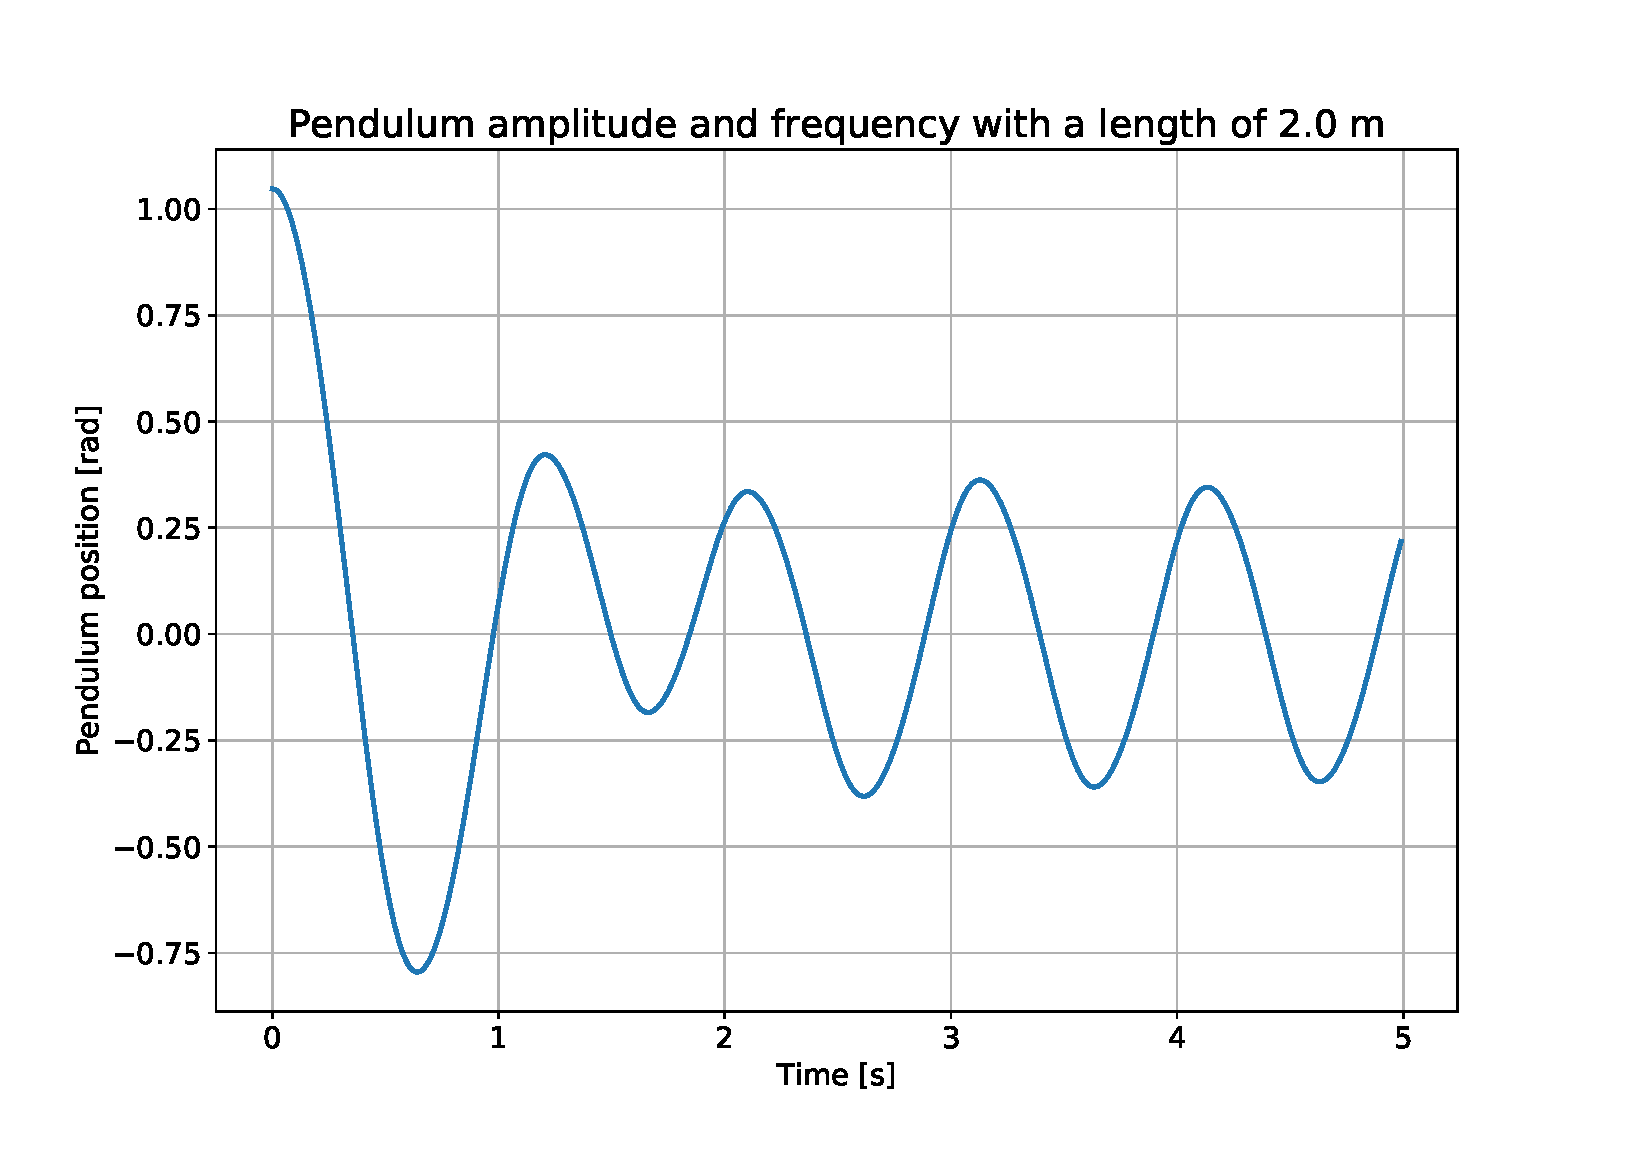
\includegraphics[height=2.5in]{len_2_0.eps}
        \caption{}
    \end{subfigure}
    \caption{ Limit cycle simulations for a pendulum of fixed mass (m=10 kg) and length of 0.5 m (a) and 2m (b). In both cases, the equilibrium position is still 0.0 rad since the muscles $M1$ and $M2$ are both 17 cm apart from the pivot point. In both cases, the limit cycle frequency is 1 Hz but the amplitudes are different.}
    \label{figure:3d_1}
\end{figure}

Then, we did the same maneuver, but that time we fixed the length at 0.5 meters (see Figure \ref{figure:3d_2}), but proceeded to simulate the limit cycle for a mass of 150 kg (a) and another of 1 kg (b). In this case, the inertia is bigger in (a) than in (b). As for Figure \ref{figure:3d_1} and for the exact same reasons, a greater inertia causes the pendulum to have a bigger initial amplitude at the first drop as compared to a lower inertia, but a smaller limit cycle amplitude. The stabilization also occurs faster for the smaller inertia pendulum, as before, and the limit cycle's oscillatory frequency is the same for both conditions.

However, notice that in Figure \ref{figure:3d_2} (b), the small irregularities observed in the curve of Figure \ref{figure:3d_1} (a) have disappeared, even though the inertia is smaller than the default case -- where the mass is 10-fold greater -- as opposed to the Figure \ref{figure:3d_1} (b) where the inertia was bigger than the default case. From this, we can deduce that Figure \ref{figure:3d_1} (b) and Figure \ref{figure:3d_2} (a) show an oscillatory system where the trajectory is more influenced by the pendulum's big inertia, that muscles struggle to counter as efficiently as they do in Figure \ref{figure:3d_2} (b), where the the notch in the trajectory shortly after time = 0 imply that the pendulum hardly opposes a resistance against the muscles action and that they govern the limit cycle trajectory.

\begin{figure}[h!]
    \centering
    \begin{subfigure}[t]{0.5\textwidth}
        \centering
        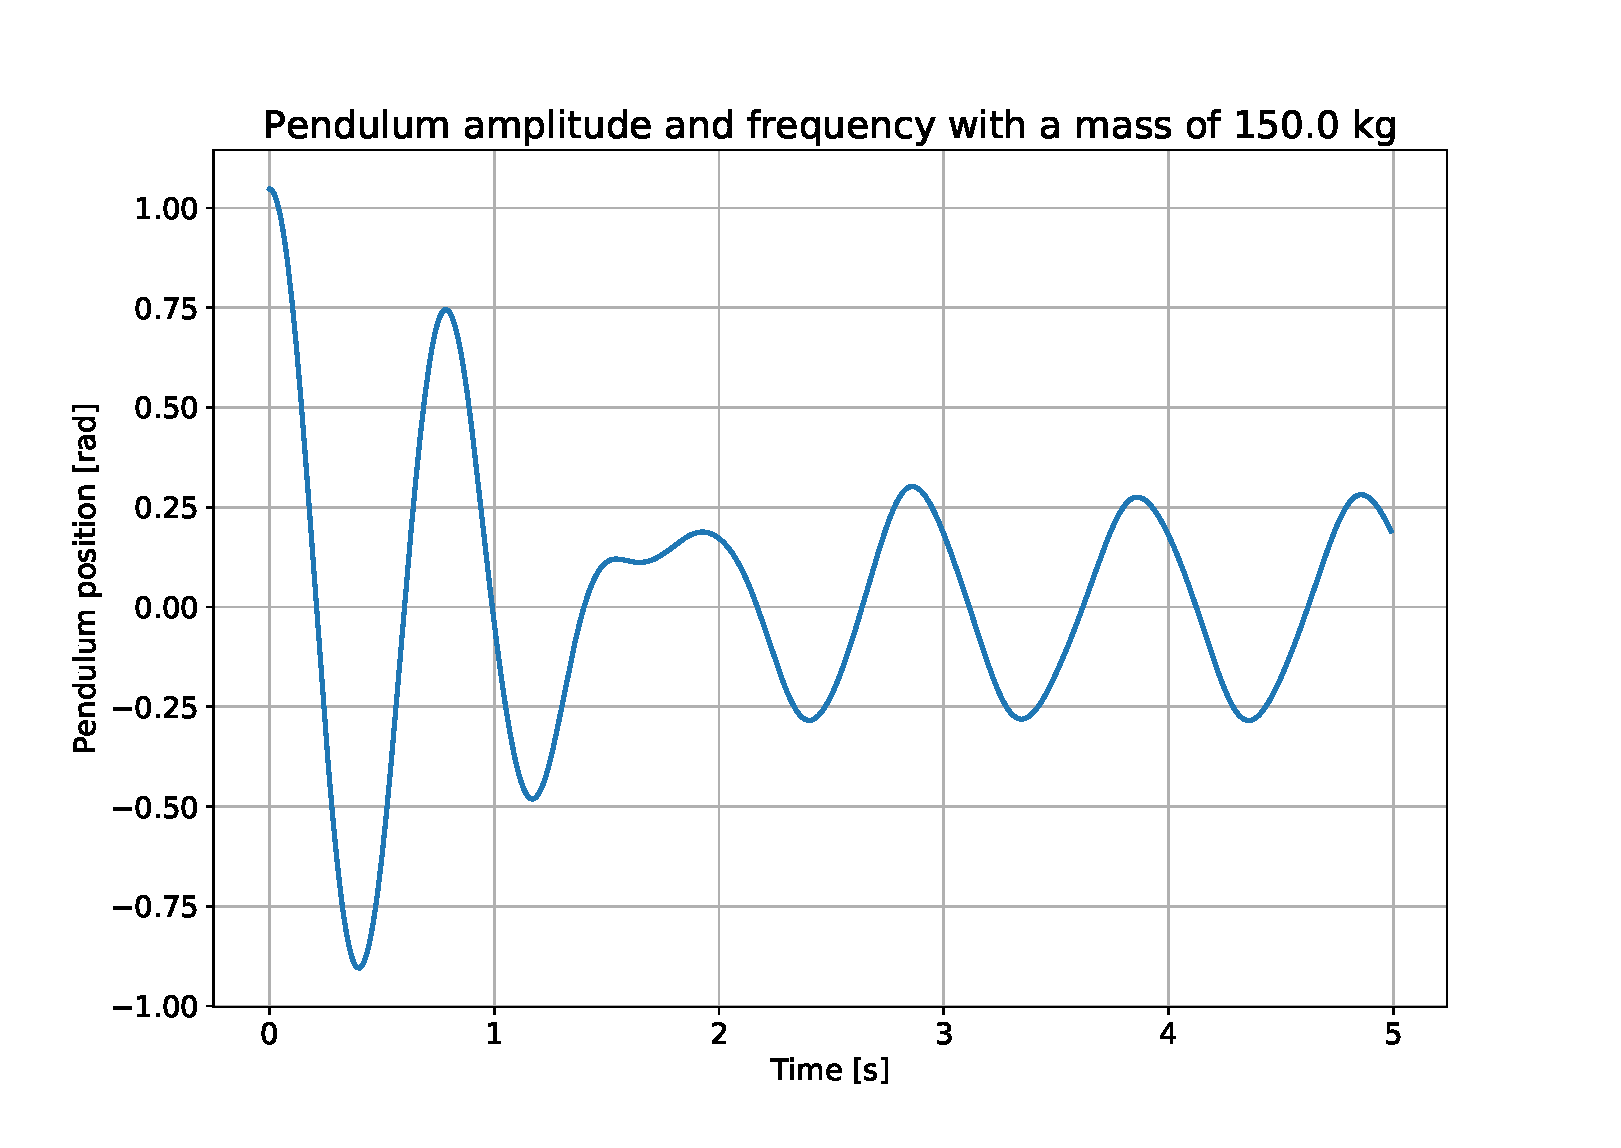
\includegraphics[height=2.5in]{mass_150.eps}
        \caption{}
    \end{subfigure}%
    ~ 
    \begin{subfigure}[t]{0.5\textwidth}
        \centering
        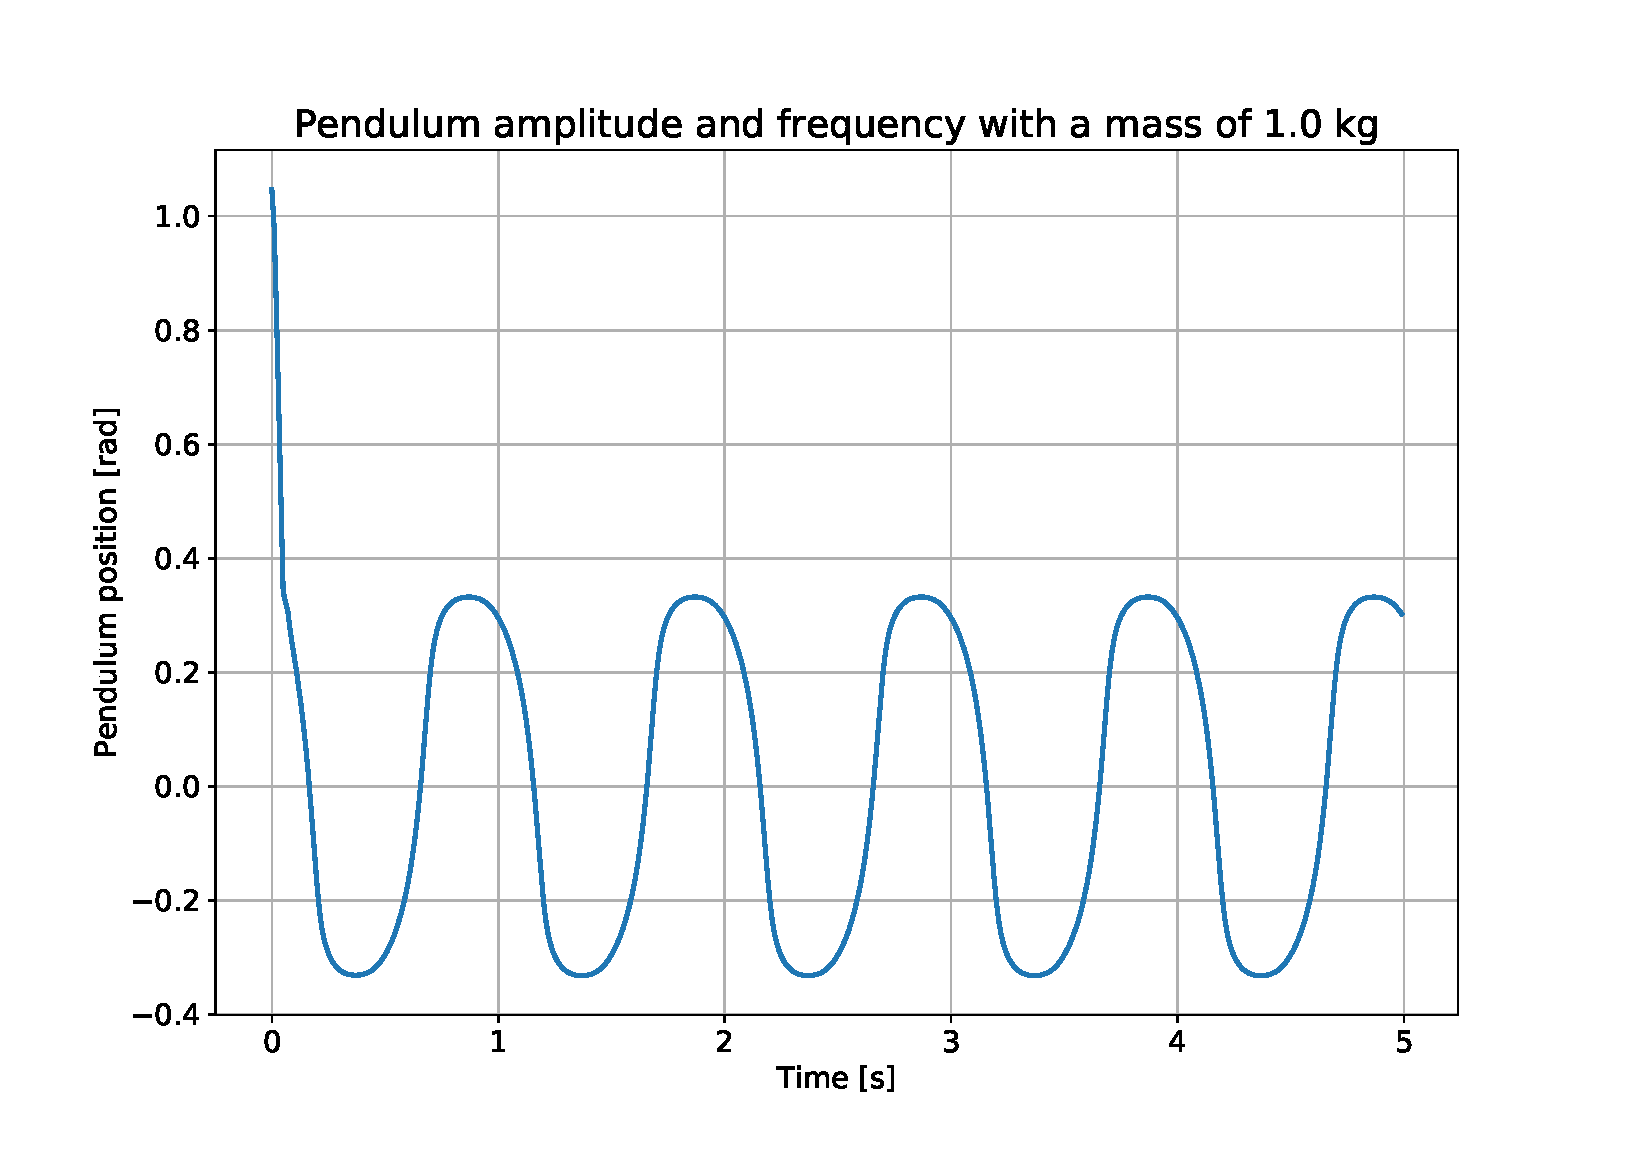
\includegraphics[height=2.5in]{mass_3.eps}
        \caption{}
    \end{subfigure}
    \caption{ Limit cycle simulations for a pendulum of fixed length (l=0.5 m) and mass of 150 kg (a) and 1 kg (b). In both cases, the equilibrium position is still 0.0 rad since the muscles $M1$ and $M2$ are both 17 cm apart from the pivot point. In both cases, the limit cycle frequency is 1 Hz but the amplitudes are different.}
    \label{figure:3d_2}
\end{figure}

\subsection*{3e. Discuss the relationship between stimulation
  frequency and amplitude with the resulting pendulum's behavior.}
\label{sec:3e}

As the above results suggest and considering these specific aspects, in order to tune the system to ones desired dynamics, one has to mitigate both the effect of the pendulum's inertia and the muscles activation frequency. Indeed, for an inertia sufficiently high with respect to the muscles activation, these won't have a significant effect to refrain the pendulum's inertia, which will preferentially force it to its equilibrium position and go against the movement that muscles are supposed to generate. In other words, for a high activation frequency and a high pendulum inertia, the muscles won't have enough time to generate a torque to counteract the torque due to inertia.

Conversely, for a sufficiently small enough pendulum's inertia, a high muscles' activation frequency will have enough time to counteract inertia and thus will contribute more to the system's dynamics!.

\subsection*{3f. Show how the pendulum's behavior is affected by the
  maximal muscle force $F_{max}$ for a given stimulation.}
\label{sec:3f}

We have shown before that the pendulum's inertia and muscles' activation have a strong influence upon each other, intermediating via the torque that either one of the others can generate. Of course, torque depends on force. In order to assess the influence of the maximum force $F_{max}$ that the muscles are capable of generating and its influence on the overall oscillatory behaviour, we simulated the limit cycle for a fixed mass (10 kg), a fixed length (0.5 m) and a maximum force of $F_{max} = 200$ N or $F_{max} = 1500$ N -- see Figure \ref{figure:3f}. In Figure \ref{figure:3f} (b), which corresponds to the default case, we observe the same dynamics as for the previous cases. In Figure \ref{figure:3f} (a) however, we observe a larger amplitude right after the drop as compared with the default case and a smaller one in the limit cycle, as for the case where the muscles couldn't counter the pendulum's inertia in Figure \ref{figure:3d_1} (b) and Figure \ref{figure:3d_2} (a). As a matter of fact, torque is defined as the product of inertia with angular acceleration, or as that of force and moment arm, such that:

\begin{equation}
\tau = I\cdot\alpha = F\cdot h.
\end{equation}

Understanding what is happening in Figure \ref{figure:3f} (a) is hence quite straightforward: when the muscles maximum force $F_{max}$ is too low with regard to the pendulum's inertia which has a greater contribution to the system's behavior, but the oscillations are still damped by the muscles and thus the inertia reduces -- since there is a negative angular acceleration -- until the point where the pendulum's inertia isn't big enough and its contribution  drops below that of the force generated by the muscles, which corresponds to the moment where the system enters a limit cycle behavior (at around 1 second in Figure \ref{figure:3f} (a)). To conclude, we can say that for a big enough $F_{max}$, one expects the limit cycle to take place faster in the time-course and be governed by the muscles more than the pendulum's inertia. 

\begin{figure}[h!]
    \centering
    \begin{subfigure}[t]{0.5\textwidth}
        \centering
        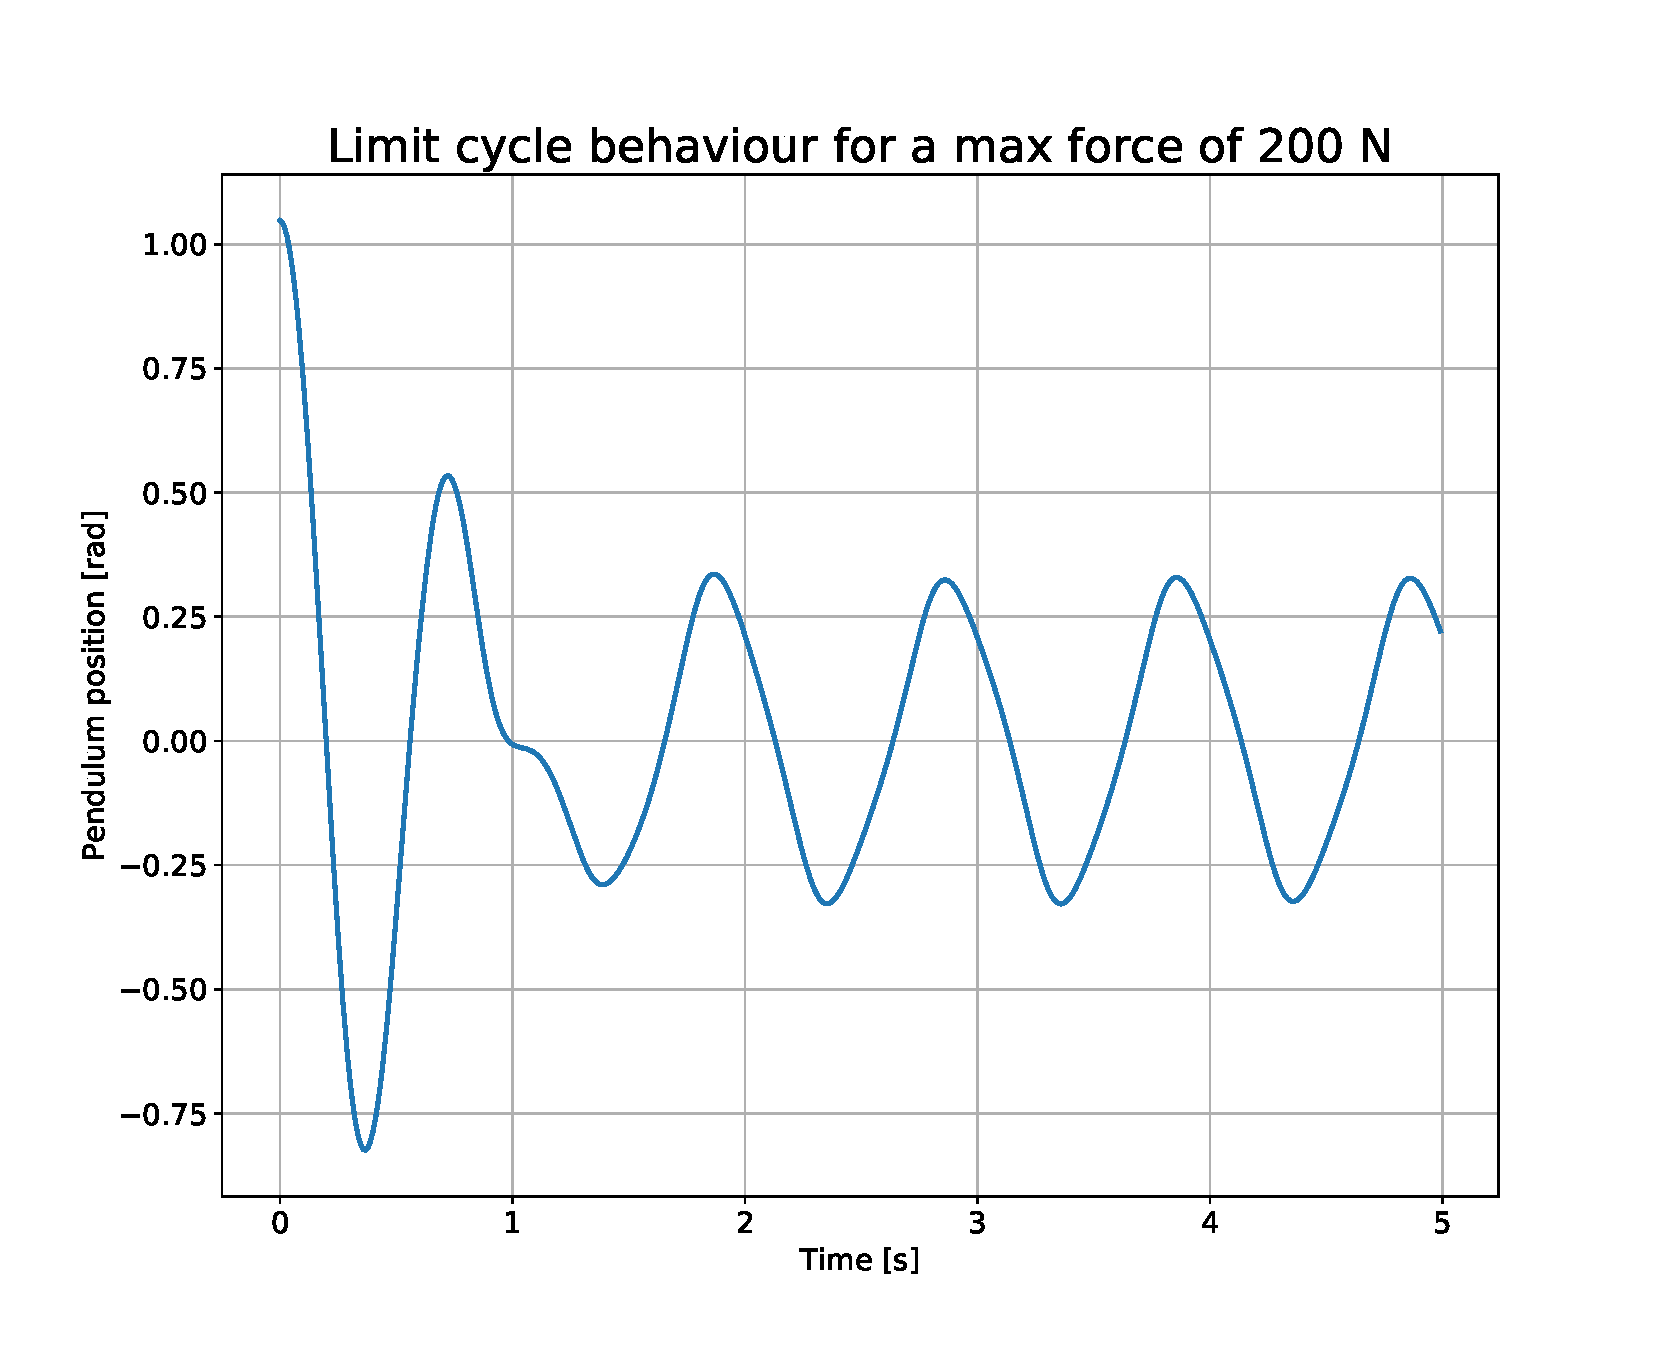
\includegraphics[height=2.5in]{200N.eps}
        \caption{}
    \end{subfigure}%
    ~ 
    \begin{subfigure}[t]{0.5\textwidth}
        \centering
        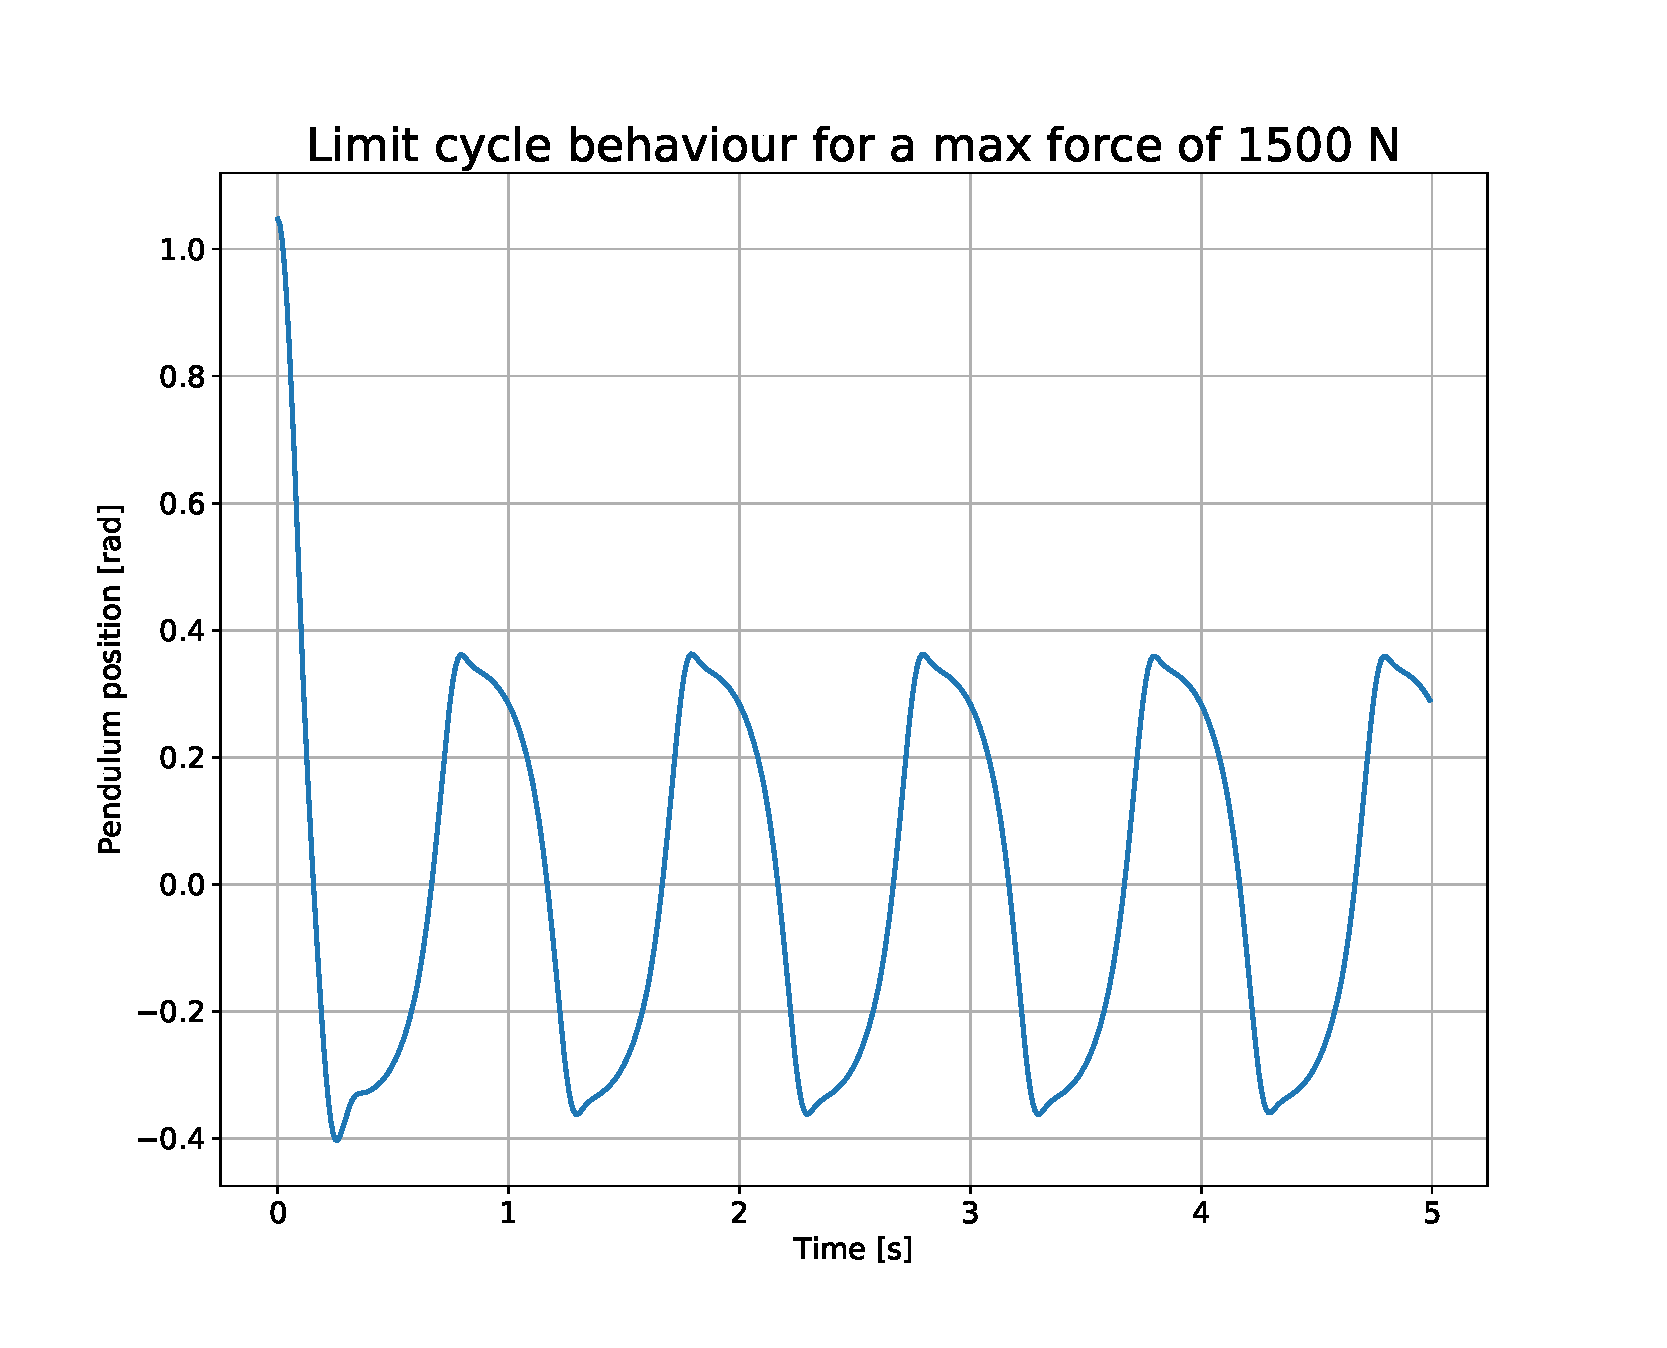
\includegraphics[height=2.5in]{1500N.eps}
        \caption{}
    \end{subfigure}
    \caption{ Limit cycle simulations for a pendulum of fixed length (l = 0.5 m) and mass  (m = 10 kg) and a maximal muscular force of  $F_{max} = 200$ N (a) or $F_{max} = 1500$ N (b). In both cases, the equilibrium position is still 0.0 rad since the muscles $M1$ and $M2$ are both 17 cm apart from the pivot point. In both cases, the limit cycle frequency is 1 Hz but the amplitudes are different.}
    \label{figure:3f}
\end{figure}

\newpage
\section*{Exercise 4 : Neural network driven pendulum model with
  muscles}
\label{sec:neur-netw-driv}

In this exercise, the goal is to drive the above system
\ref{fig:p_muscles} with a symmetric four-neuron oscillator
network. The network is based on Brown's half-center model with
fatigue mechanism. Here we use the leaky-integrate and fire neurons
for modelling the network. Figure \ref{fig:p_muscles_neurons} shows
the network structure and the complete system.

\begin{figure}[H]
  \centering
  \includegraphics[scale=1.5]{figures/pendulum_muscles_neurons.pdf}
  \caption{Pendulum with Antagonist Hill Muscles Driven Half Center
    Neural Network.}
  \label{fig:p_muscles_neurons}
\end{figure}

Since each leaky-integrate and fire neuron comprises of one first
order differential equation, the states to be integrated now increases
by four(one state per neuron). The states are,


\begin{equation}
  \label{eq:1}
  X = \begin{bmatrix}
    \theta & \dot{\theta} & A_1 & l_{CE1} & A_2 & l_{CE2} & m_1 & m_2 & m_3 & m_4
  \end{bmatrix}
\end{equation}

Where,

\begin{itemize}
\item $m_1$ : Membrane potential of neuron 1
\item $m_2$ : Membrane potential of neuron 2
\item $m_3$ : Membrane potential of neuron 3
\item $m_4$ : Membrane potential of neuron 4
\end{itemize}

To complete this exercise, additionally you will have to use
\fileref{NeuralSystem.py} and \fileref{exercise4.py}

\subsection*{4a. Find a set of weights for the neural network that
  produces oscillations to drive the pendulum into a limit cycle
  behavior.}
\label{sec:4a}
Matrix \eqref{eq:weights} shows one possible example of dendritic weights that generate a limit cycle. The limit cycle is depicted in Figures \ref{Limit cycle} and \ref{Time Evolution}. Note that it takes a few seconds, around 7.5, to reach the limit cycle. It is robust against a small perturbation as shown in Figure \ref{Perturbation}, where the red dot indicates said perturbation.

\begin{mycapequ}[!ht]
\caption{Neural networks weights matrix}
\begin{equation}
\begin{pmatrix}
0 & -5 & -5 & 0 \\
-5 & 0 & 0 & -5 \\
3 & -1 & 0 & 0 \\
1 & 3 & 0 & 0 
\end{pmatrix}
\label{eq:weights}
\end{equation}
\end{mycapequ}

%\begin{table}[h]
%\centering
%\caption{Weight matrix producing an oscillation}
%\label{weights}
%\begin{tabular}{|l|l|l|l|l}
%\cline{1-4}
%0  & -5 & -5 & 0  &  \\ \cline{1-4}
%-5 & 0  & 0  & -5 &  \\ \cline{1-4}
%3  & -1 & 0  & 0  &  \\ \cline{1-4}
%-1 & 3  & 0  & 0  &  \\ \cline{1-4}
%\end{tabular}
%\end{table}

\begin{figure}[H]
  \centering
  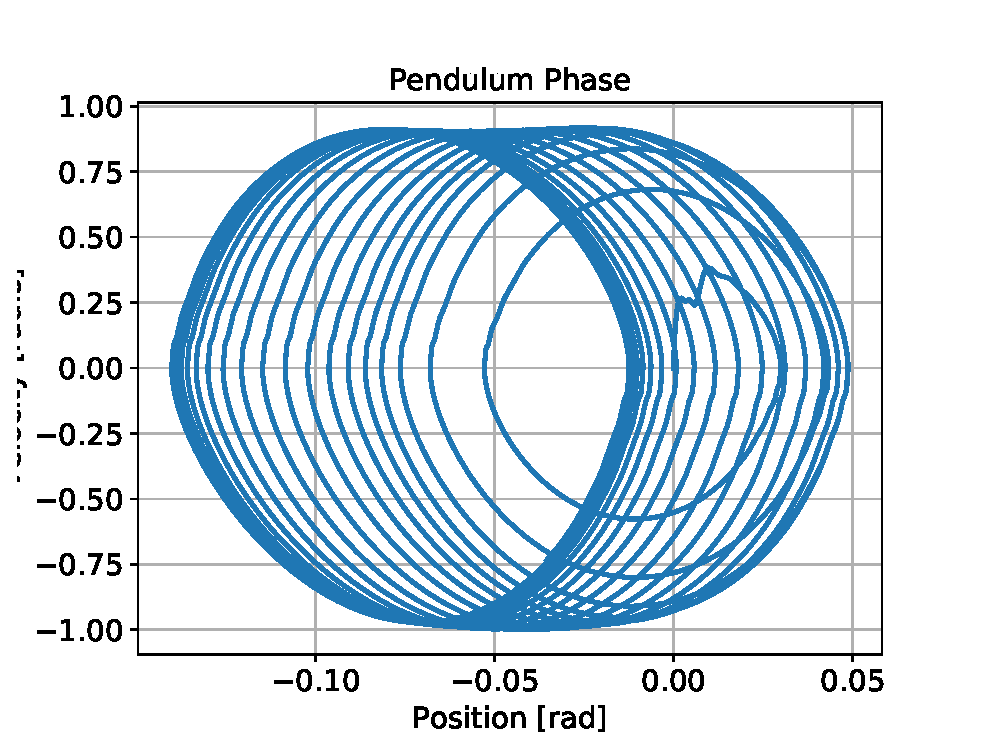
\includegraphics[scale=0.75]{FirstCycle.eps}
  \caption{Phase portrait of the pendulum receiving activation by a neuron system. The neuron system has the connection parameter depicted in Matrix \eqref{eq:weights}. Bias and time constants of neurons are respectively (3, 3, -3, -3) and (0.02 s, 0.02 s, 0.1 s, 0.1 s). Pendulum length and mass are respectively 50 cm and 1 kg. Simulation time is 10 s with steps of 0.001 s.}
  \label{Limit cycle}
\end{figure}
\begin{figure}[H]
  \centering
  \includegraphics[width=0.6\textwidth]{FirstTime_Phase.eps}
   \caption{Evolution of position and velocity of the system related to Figure \ref{Limit cycle}. The center of the cycle limit is approximately -0.075 rad and its frequency is approximatively 2 Hz with an amplitude of 0.13 rad.}
  \label{Time Evolution}
\end{figure}


\begin{figure}[H]
  \centering
  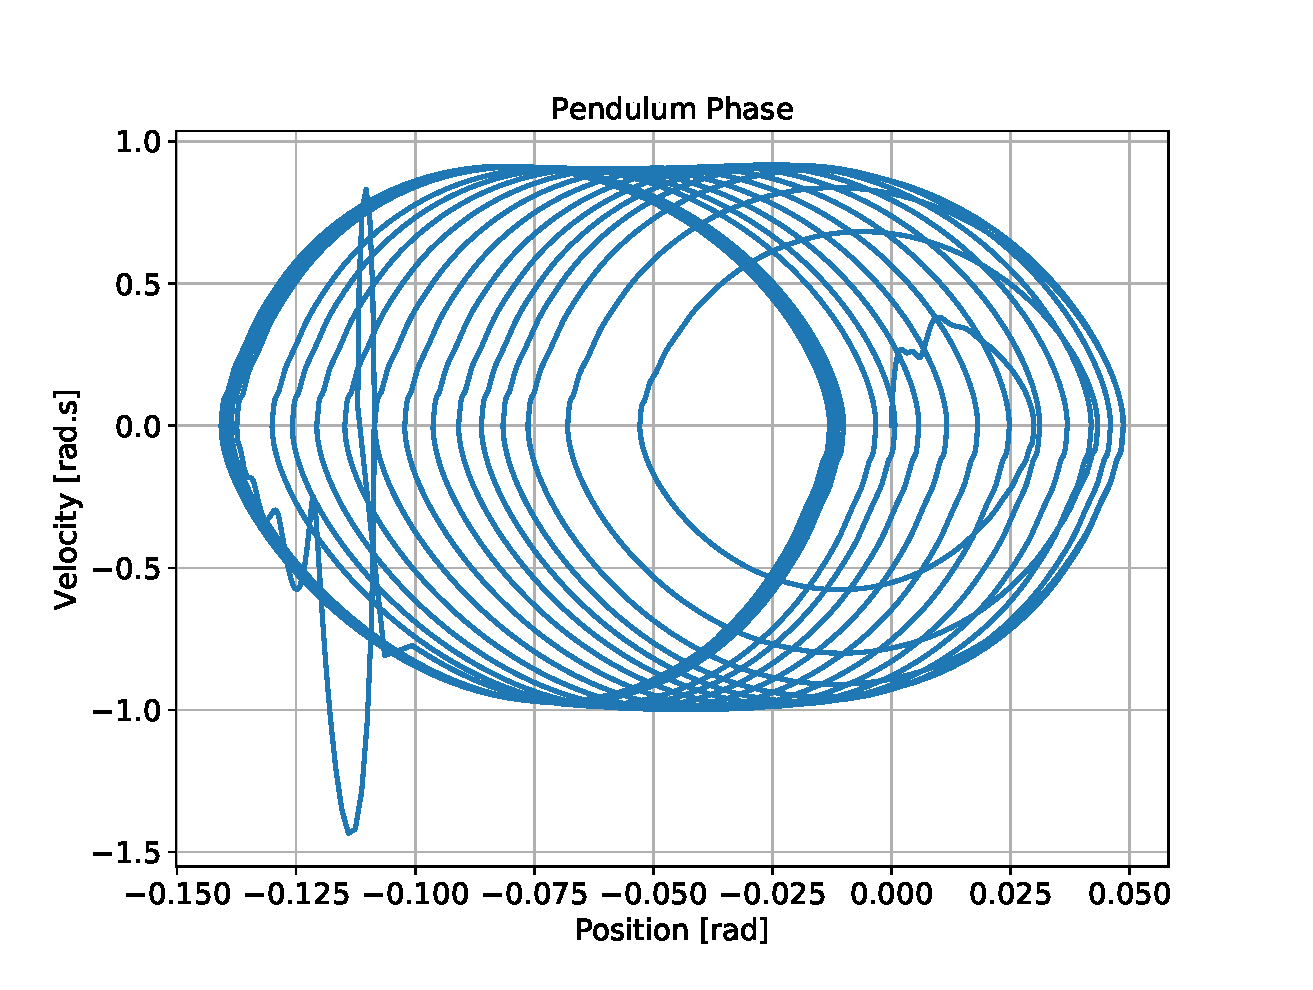
\includegraphics[width=0.8\textwidth]{WithASmallPerturbation.eps}
  \caption{Same as Figure \ref{Limit cycle} but with a small perturbation of position and speed at 7 s, marked here as a red dot. After the perturbation, the system reaches back to the same trajectory pattern as previous to the perturbation.}
  \label{Perturbation}
\end{figure}

\subsection*{4b. Show how the network weights, bias and time constant
  parameters affect the behavior of the pendulum.}
\label{sec:4b}

Increasing all biases at the same time can increase the cycle frequency since we facilitate the neuron activation by shifting the activation sigmoid curve to the left, implying that activating the neuron will require a smaller amount of dendritic input, but this holds only up to a certain point. Indeed, for too high bias increases, the frequency drops (see Figure \ref{Biases}). This is due to the fact that when we facilitate the neuronal activation too much, the neurons aren't as efficient in counteracting the system's inertia. Concerning the opposite phenomenon, when decreasing the biases, the frequency drops as we shift the activation curve to the right, implying that a higher dendritic sum is required for the neuron to be active. Concerning the amplitude, when the biases are decreased by -0.9, the amplitude is higher than the situation where the shift is +4.85. Furthermore, modifying one  bias at a time will significantly shift the equilibrium position as we only facilitate or incapacitate one neuron at a time (data not shown). 

Increasing time constants $\tau$ decreases the cycle frequency, as shown in Figure \ref{taus}. This is due to the fact that a bigger time constant will cause the the membrane potential of the virtual neurons to change more slowly, hence implying that the whole system will have a slower response to a change in the neuronal dynamics. 

Multiplying weights also increases both frequency and amplitude, as shown in Figure \ref{multiweight}: indeed, by doing that we increase the contribution of the neuronal inputs to the system's dynamics and overcome the system's inertia more efficiently. Noticeably, when setting up too small weights, no limit cycle will occur, as the influence of the neurons as compared to the inertia of the system will be just sufficient enough to generate perturbations, but not big enough to entrain the pendulum in a limit cycle behavior (data not shown).
\begin{figure}[H]
\centering
 \begin{subfigure}[t]{0.5\textwidth}
  \centering
  \includegraphics[scale=0.5]{biases/Plus02.eps}
  \caption{All biases shifted by +0.2.}
 \end{subfigure}
 ~
 \begin{subfigure}[t]{0.4\textwidth}
 	\centering
 	\includegraphics[scale=0.4]{biases/minus09Time_Phase.eps}
 	\caption{All biases shifted by -0.9.}
 \end{subfigure}
 
 \begin{subfigure}[t]{0.5\textwidth}
 	\centering
    \includegraphics[scale=0.4]{biases/Plus4_85Time_Phase.eps}
    \caption{All biases shifted by +4.85.}
  \end{subfigure}
  \caption{Biases in the reference cycle from Figure \ref{Limit cycle} are, respectively for each neuron, [3, 3, -3, -3] and here the biases are either shifted downwards or upwards. For a +0.2 shift, the frequency increases slightly as compared with the limit cycle obtained before, but with more extreme value such +4.85, the frequency drops drastically. For a -0.9 reduction of all biases, the frequency is also reduced. The amplitude for biases decreased by -0.9 is 0.1 rad and 0.15 for a +4.85 increase. With high positive shift, the neurons 3 and 4 are almost always active, whereas for negative shifts, they are deactivated.}
  \label{Biases}
\end{figure}


\begin{figure}[H]
  \centering
  \begin{subfigure}[t]{0.5\textwidth}
  	\centering
  	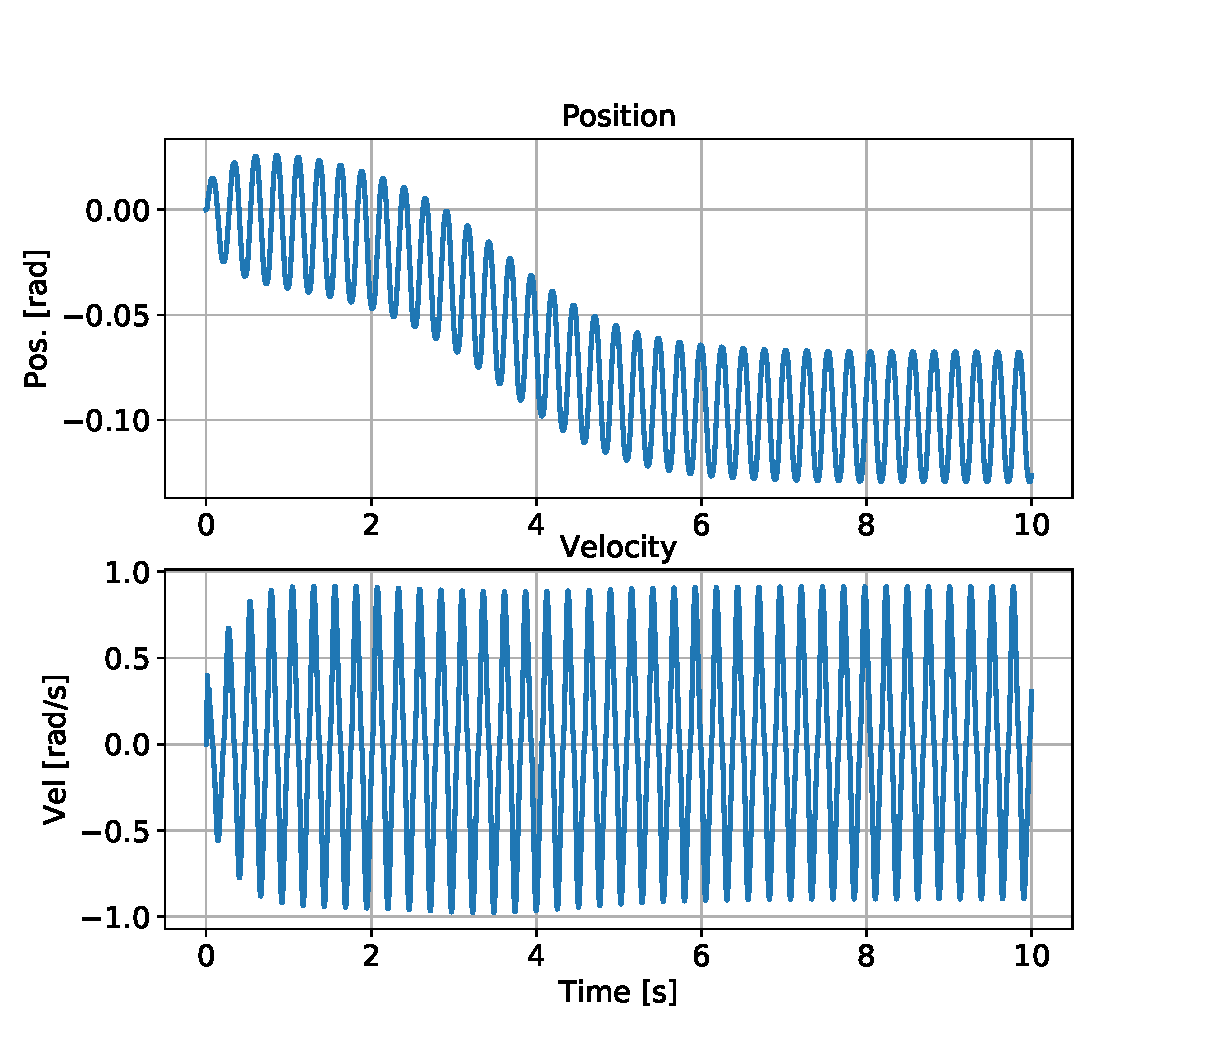
\includegraphics[scale=0.4]{allTaudividedby2.eps}
    \caption{All $\tau$'s divided by 2.}
  \end{subfigure}
  ~
  \begin{subfigure}[t]{0.4\textwidth}
  	\centering

  	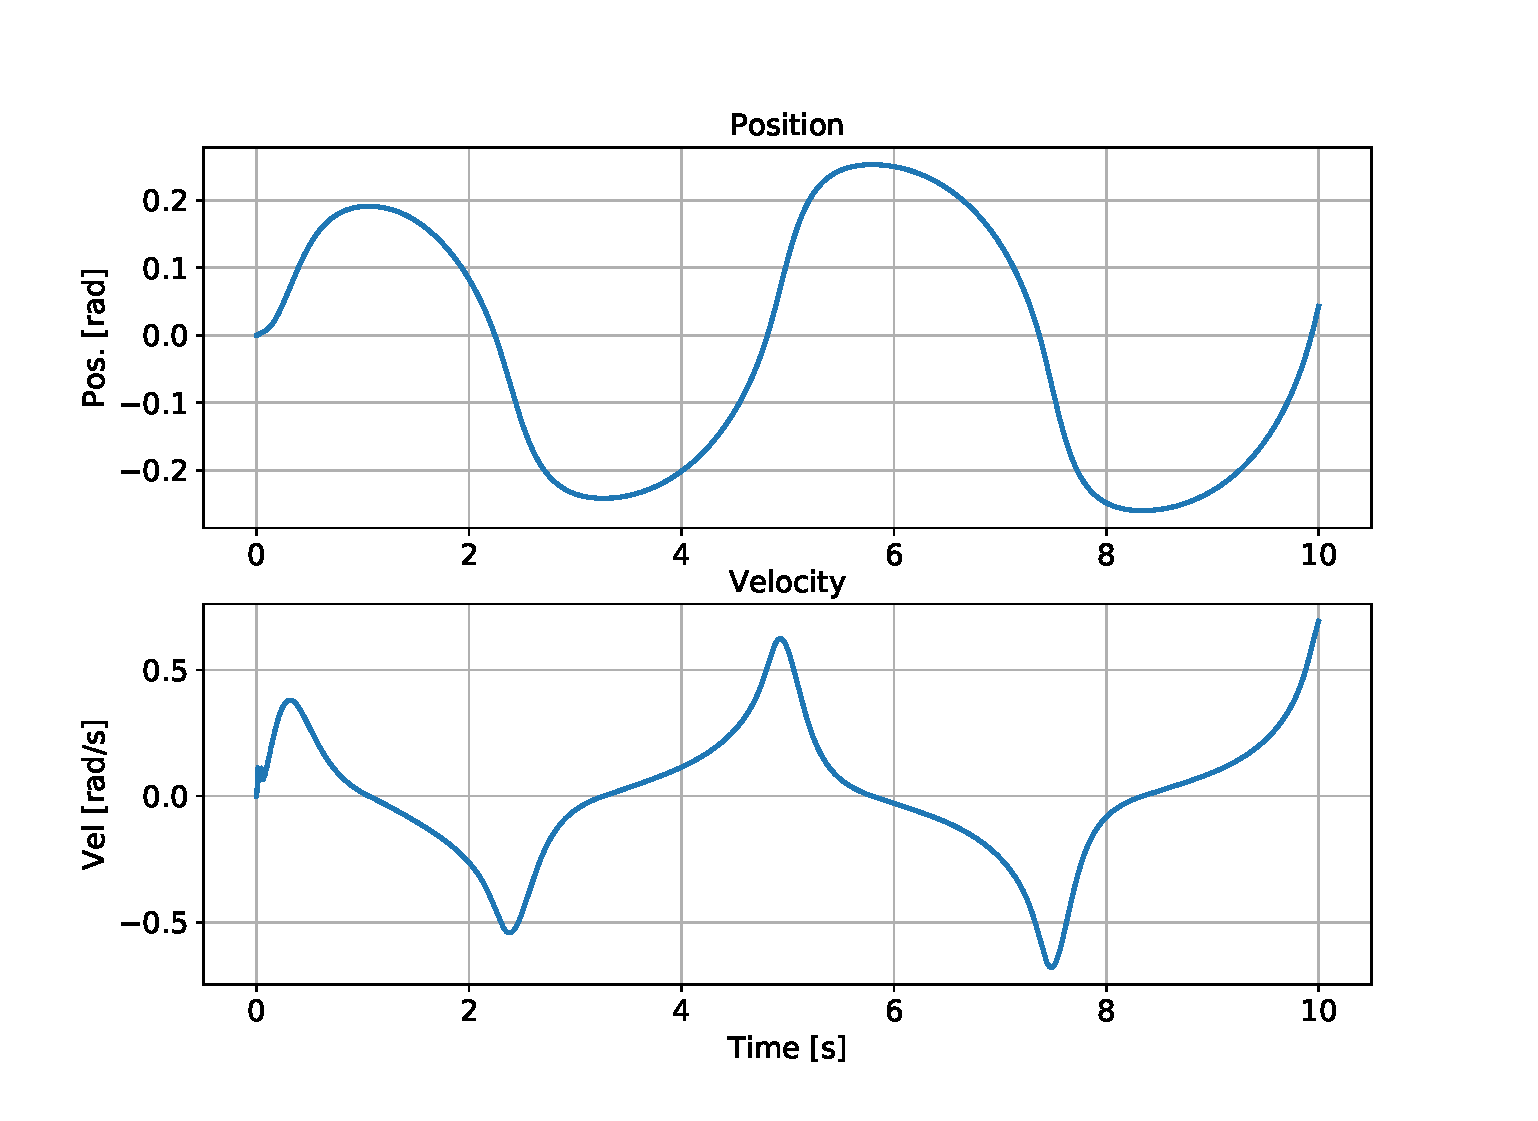
\includegraphics[scale=0.35]{allTauMultipliedBy10.eps}
    \caption{All $\tau$'s multiplied by 10.}
   \end{subfigure}
  \caption{The parameters are the same as those of Figure \ref{Limit cycle}, but the time constants $\tau$'s were all multiplied or divided. With smaller $\tau$'s, the frequency is 4 Hz, higher than the reference limit cycle of Figure \ref{Limit cycle} which is 2 Hz. When they are bigger, the frequency is approximatively 0.3 Hz. }
  \label{taus}
\end{figure}

\begin{figure}[H]
\centering
\includegraphics[scale=0.7]{biases/weights2x.eps}
\caption{Weights of matrix \ref{eq:weights} are all multiplied by 2. The frequency is 4.5 Hz against 2 Hz for the reference limit cycle and the oscillations are higher than our reference cycle in Figure \ref{Time Evolution}. The center of limit cycle is 0.0 here.}
\label{multiweight}
\end{figure}

\subsection*{4c.As seen in the course, apply an external drive to the
  individual neurons and explain how the system is affected. Show
  plots for low [0] and high [1] external drives. To add external
  drive to the network you can use the method \\
  \fileref{SystemSimulation.py::add\_external\_inputs\_to\_network} }
\label{sec:4c}

As seen in the course, applying an external drive can change the frequency. An excitatory drive will most likely cause the neurons to activate at a higher rate. In order to assess this, we simulated the non-driven case we studied until now and suddenly applied an external drive of 1 to the system. The results shown in Figures \ref{DD1} and \ref{DD2} demonstrate that the limit cycle frequency increases and the amplitude decreases as an external drive equal to 1 is added. This is consistent with what we have studied in the course and could be useful in order to simulate some kind of descending drive from the brain stem or even an environmental feedback, to some extent. A visual simulation of this sudden drive addition is available at \url{https://www.youtube.com/watch?v=EEUjSFnY7Zs}.

\begin{figure}[H]
  \centering
  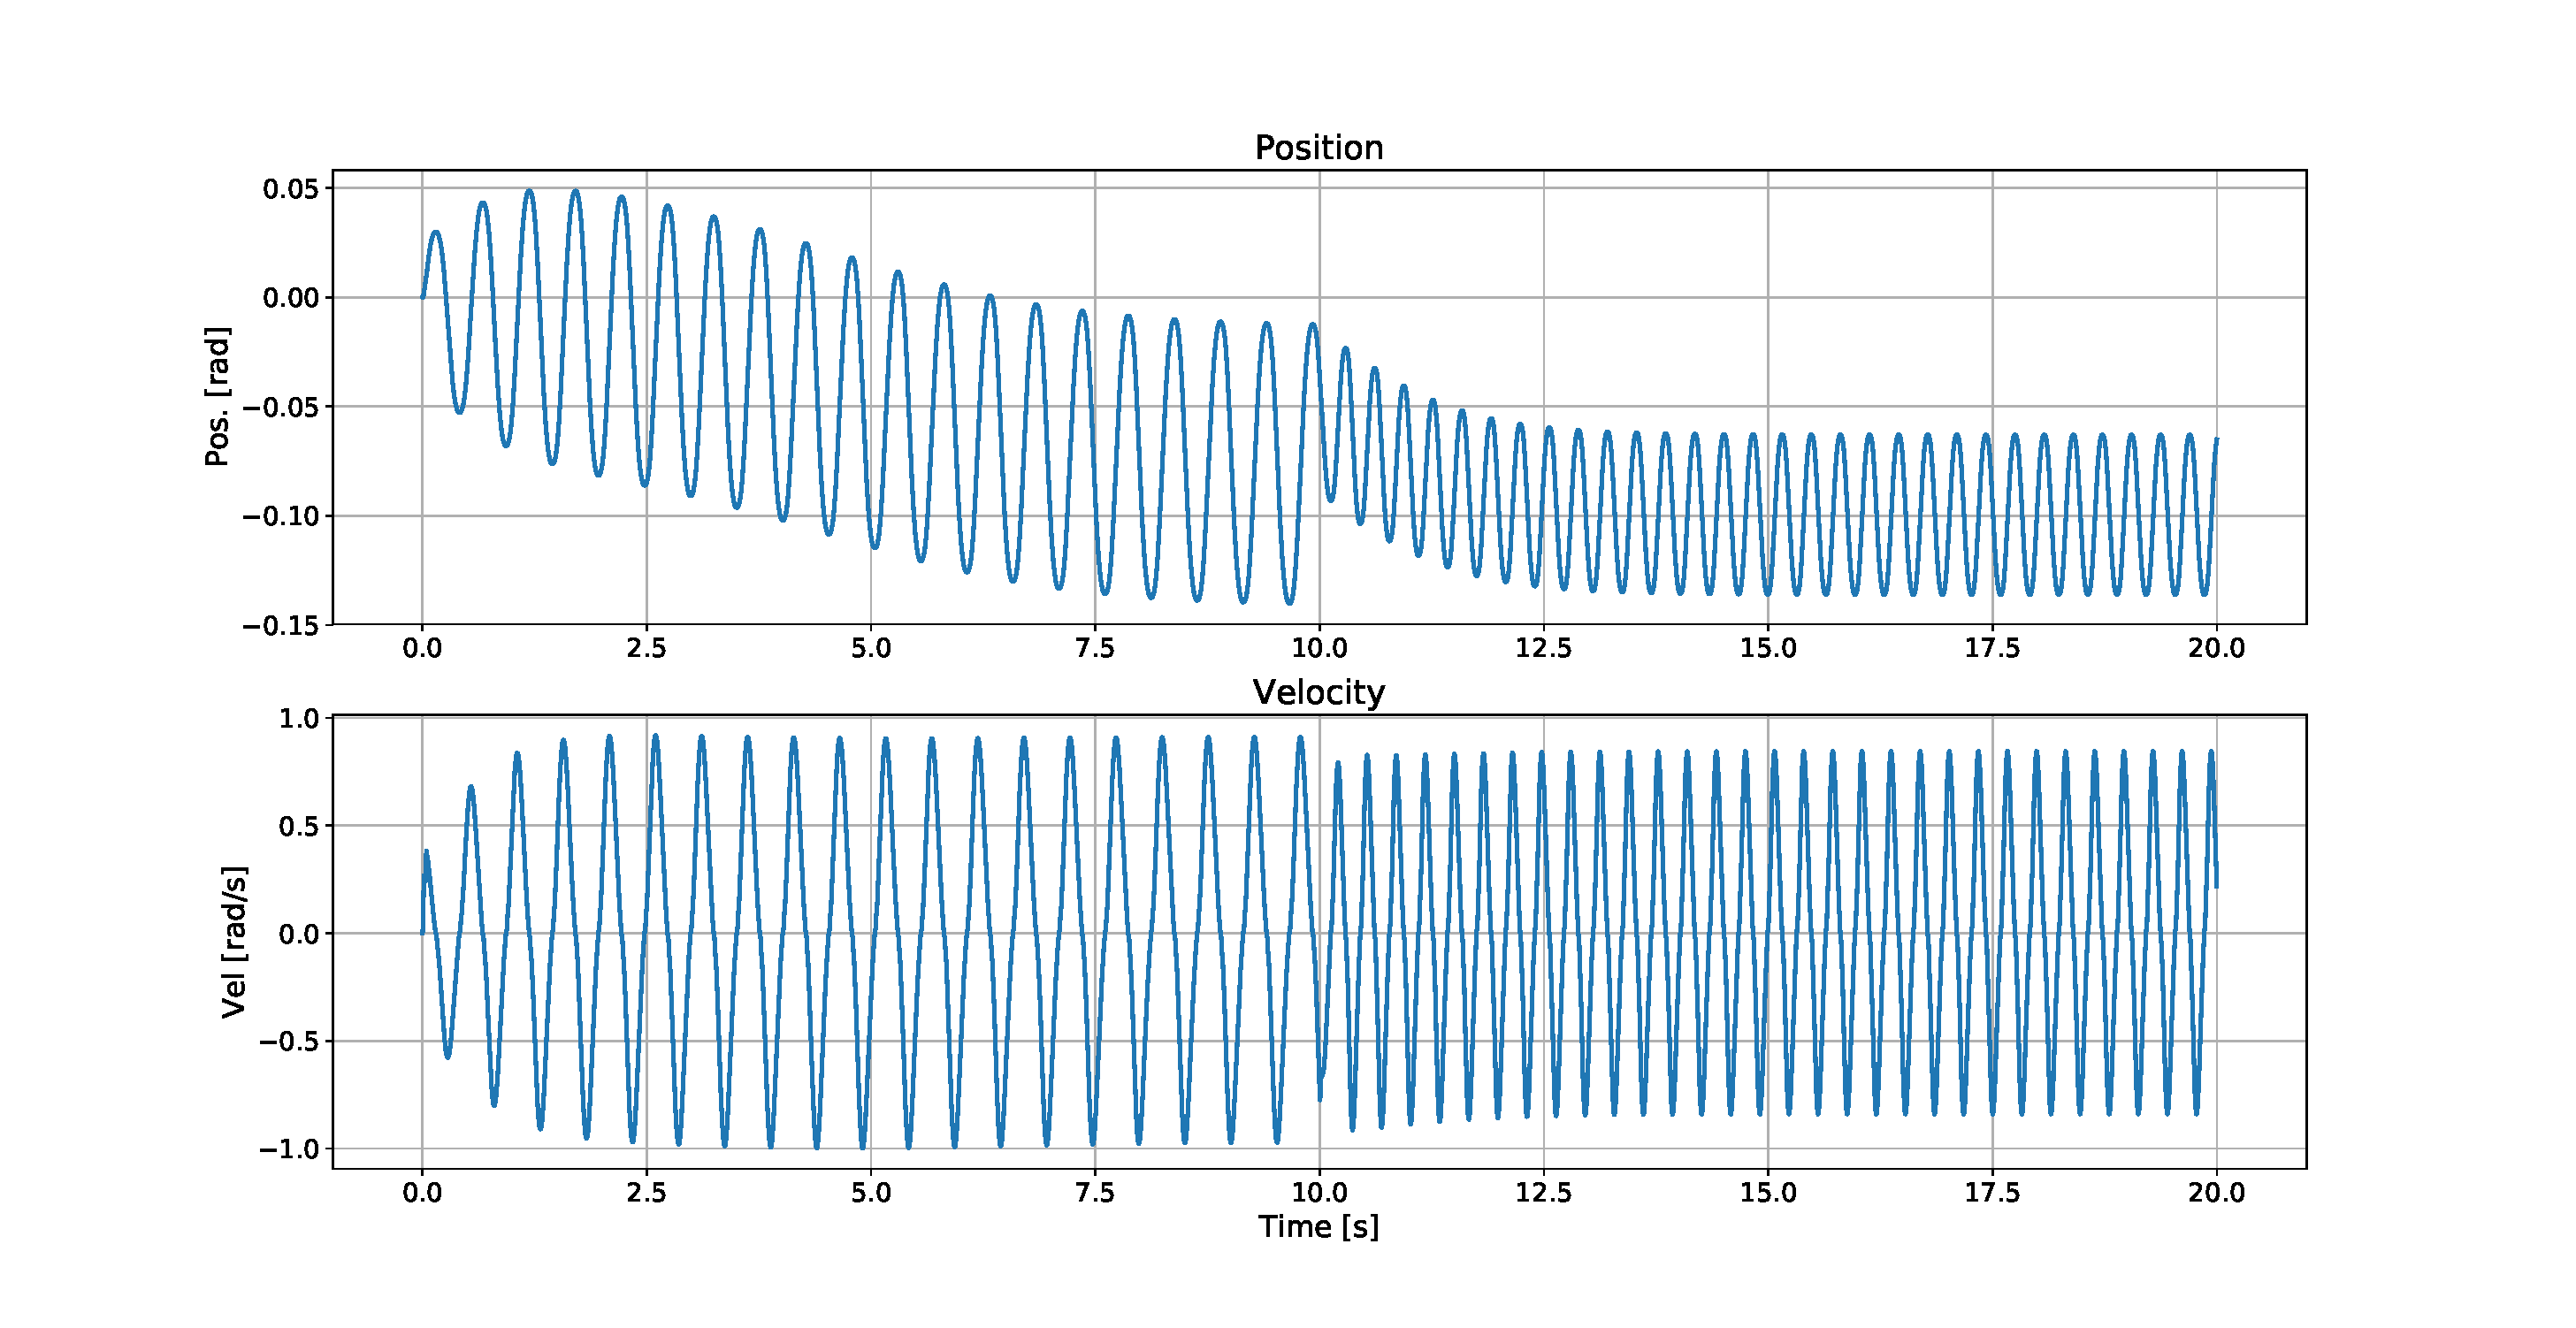
\includegraphics[width=1\textwidth]{ExternalDrivePosVel.eps}
  \caption{Same as Figure \ref{Time Evolution} but we added an external drive of 1 at half the simulation time (time = 10 s). Frequencies are different: 2 Hz when there isn't any external drive against 3 Hz for an external drive of 1. Amplitude is two times smaller with the activation, and the equilibrium position has shifted to -0.1.}
  \label{DD1}
\end{figure}

\begin{figure}[H]
  \centering
  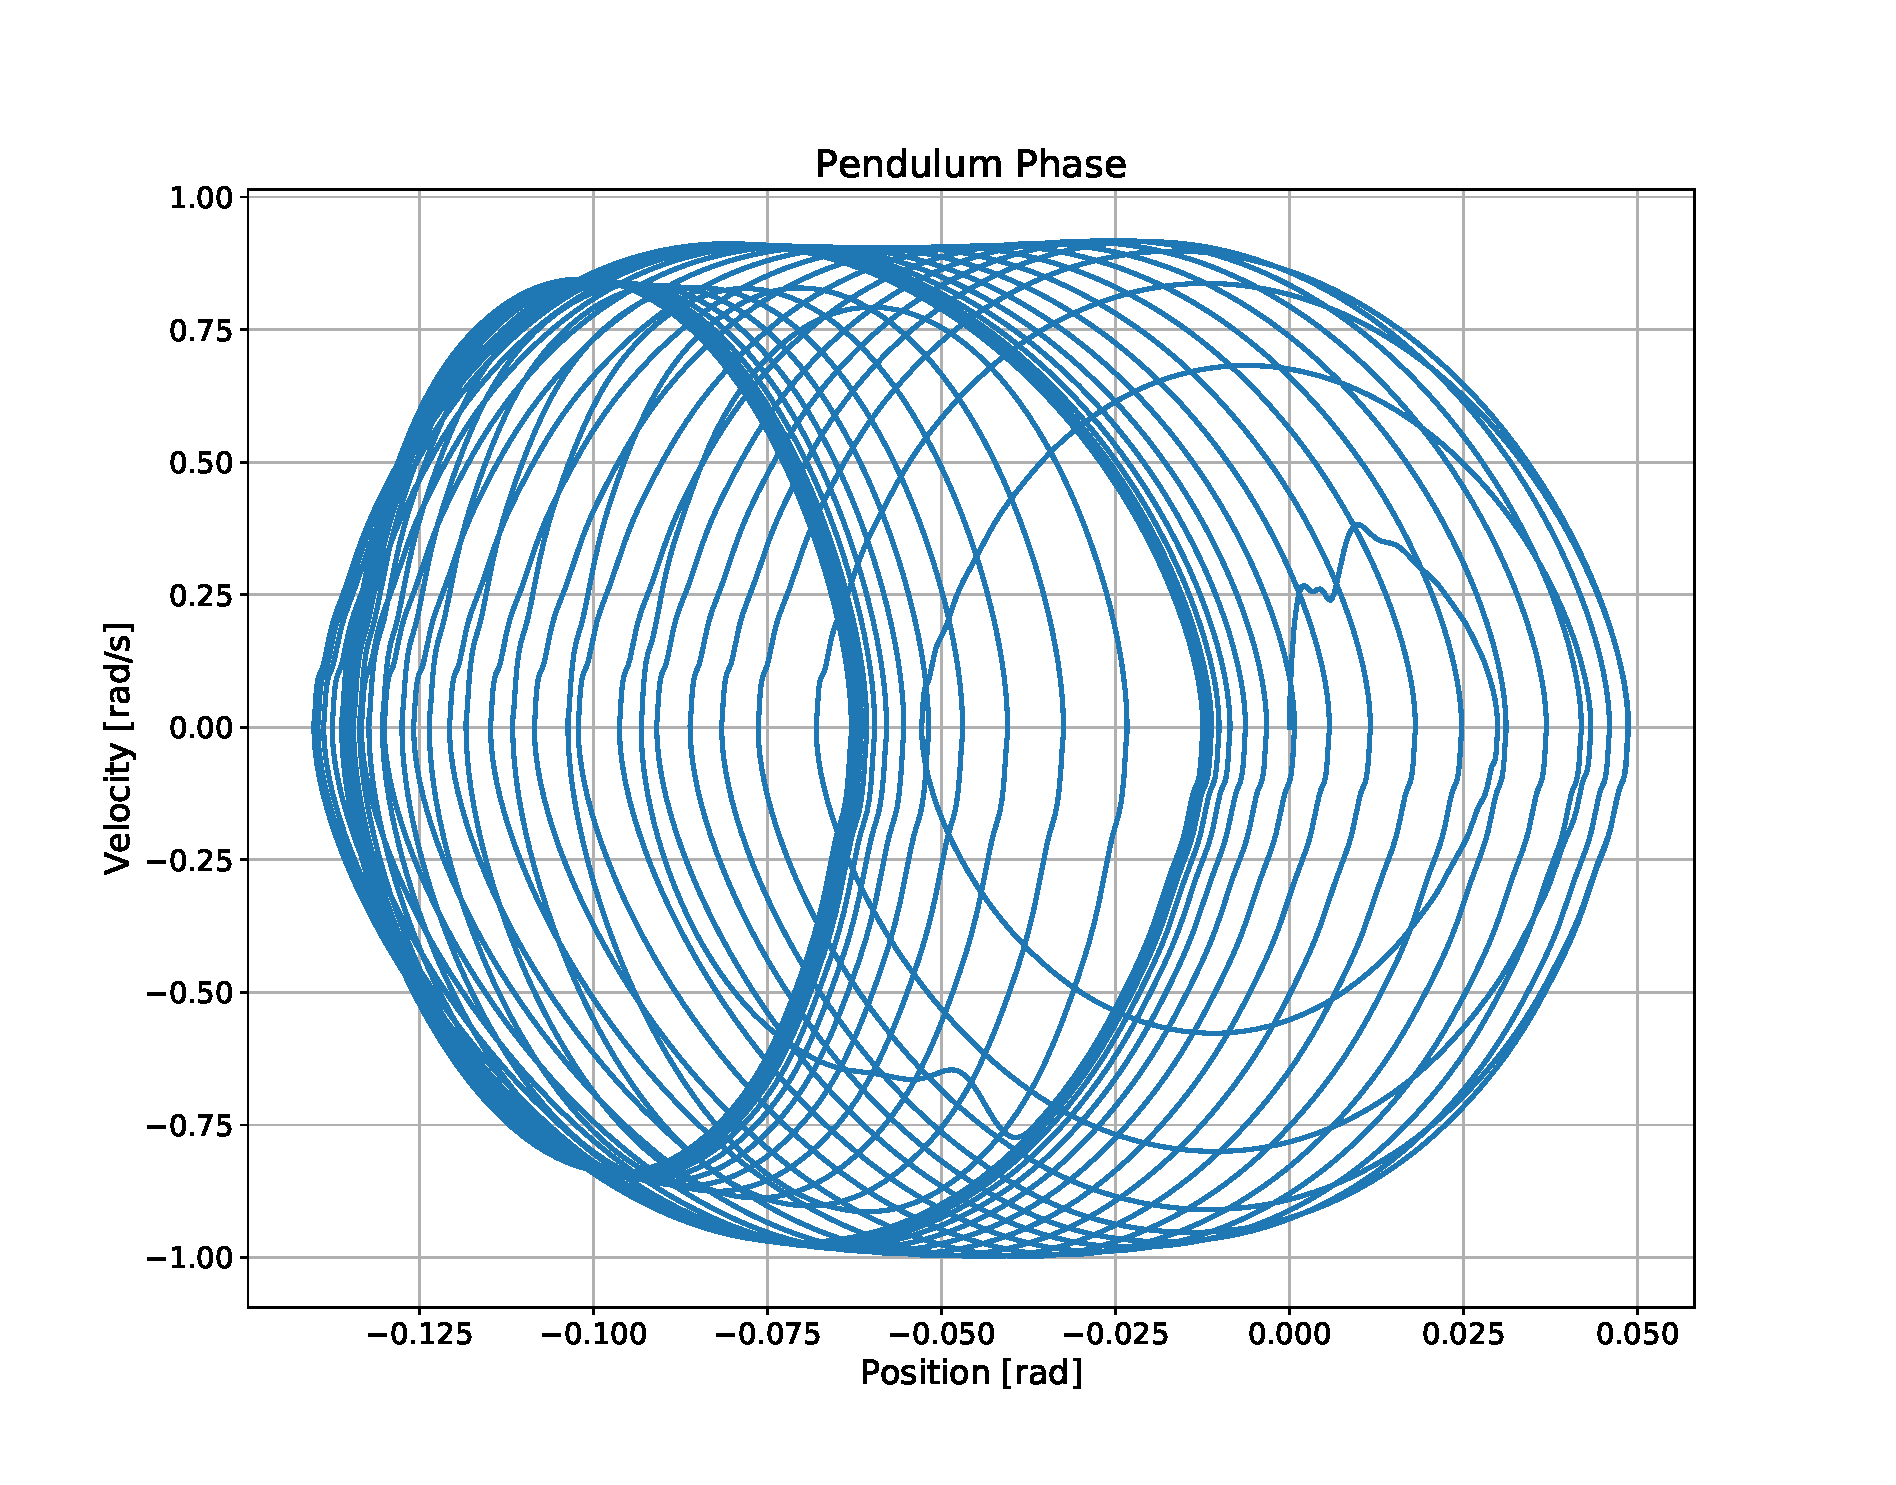
\includegraphics[width=0.8\textwidth]{ExternalDrivePhase.eps}
  \caption{Same as Figure \ref{Limit cycle} but we added an external drive of 1 at half the simulation time (time = 10 s). Frequencies are different: 2 Hz when there isn't any external drive against 3 Hz for an external drive of 1. Amplitude is two times smaller with the activation, and the equilibrium position has shifted to -0.1.}
  \label{DD2}
\end{figure}

\newpage
\subsection*{4d. [Open Question] What are the limitations of the half center model in
  producing alternating patterns to control the pendulum? What would
  be the effect of sensory feedback on this model?}
\label{sec:4d}

As we have seen it, we were able to generate quite steady limit cycles, and were even able to switch between different limit cycles with different frequencies and amplitudes. Whereas this does not pose any issue in the context of a single oscillating pendulum, the cycles that we could generate with a multiple-oscillators model based on half-centers might be a little too formal and regular, preventing us to simulate the more realistic movement of a typical articulation such as that of the knee, which can involve irregular and different limit cycles for each part of the system  -- e.g. a pause of one pendulum (thigh) while the other performs an oscillation (shin).

% As we have seen in it during the lectures with the example of the salamander, neurons governing a certain pattern generator in nature will be able to achieve a transition between two types of gait depending on the external drive which they are subjected to -- low current will drive the animal into walking and high current will cause it to switch to swimming. Using a virtual neuron model such as the leaky integrate-and-fire model implies that a neuron will be characterized by only one activation function, hence making it difficult to mimic this natural CPG behavior with only one type of neuron population.

% For one oscillator, we have a model that is able to simulate changes in limit cycle behaviors and therefore changes in the gait's pattern. But would we want to expand the model to a set of connected pendulums -- to mimic a vertebrae joint for instance -- we would likely be confronted to an incapacity to make this articulation exhibit two different types of gaits for different external drives, since our neuron population is characterized by a single type of activation function. In order to be able to make a multiple-oscillator model switch between different inter-oscillators synchronization patterns, we would have to model an additional type of neurons, characterized by different intrinsic characteristics such as synaptic weights, activation function, threshold, and more.

As to the simulation of a sensory feedback, the first approach would consist in considering it as a perturbation, since a sensory feedback can be seen as a discrete event -- e.g. stepping on a nail. After such an event, the system would just reach back to the limit cycle it was describing before. This is however in a context where a sensory feedback would be interpreted as a sort of reflex, but the definition applies to another important concept: indeed, sensory feedback can also be considered as an event taking place in a larger timescale, for instance as a constant signal telling the body/system that it is moving in water, or a periodic signal occurring for the whole duration of each steps (somatosensory feedback). Looking at it from this angle, we could implement the feedback as an external drive, which would allow us to modulate the original limit cycle into a new one, as we did in Figure \ref{DD1}. Nonetheless, switching from a stable limit cycle to another consequently to an external input takes some time (around 5 seconds in our example), and this might by a problem if we want to model a fast-reacting system closer to nature. Furthermore, this model requires to integrate four states per CPG, and this might cause even more lag-response when modeling a higher number of connected CPGs.

\end{document}

%%% Local Variables:
%%% mode: latex
%%% TeX-master: t
%%% End: